%%%%%%%%%%%%%%%
% This style of this thesis is based on the thesis proposal required to be submitted at the start of the Master's thesis project in the Artificial Intelligence program.
% It has been updated with the new high-res banner for the Faculty of Science and Engineering, and includes, among other features, a contents page, an acknowledgements page, and appendices.

% Author: Hari Vidharth
% Last modified: TBD
%%%%%%%%%%%%%%%

\documentclass[a4paper,12pt,twoside]{article}
%\documentclass[a4paper,12pt]{article}
\usepackage{comment}
\usepackage{lipsum}
\usepackage{multirow}
\usepackage{subcaption}
\usepackage{xcolor}
\usepackage{amsmath}
\usepackage{wrapfig}    % inline figures
\usepackage{enumitem}
\usepackage{mwe}
\usepackage{graphicx} % Use for Images
\usepackage{here}     % Forced Figure Placement
\usepackage{pslatex}	% Use PostScript Fonts
\usepackage{fancyhdr} % Use headers
\usepackage{float}
\usepackage{hyperref}
% Here I keep the left and right margins equal. You can choose to have unequal margins if you want a two-sided book effect.
\usepackage[
	top    = 1.5cm,
	bottom = 1.80cm,
	left   = 2.00cm,
	right  = 2.00cm,
	includeheadfoot]{geometry} % Use similar margins to the Word Template
\setlength{\parindent}{0pt}

% Define the page styles
\fancypagestyle{titlepage}{
	\fancyhf{}
	\fancyhead[C]{
\includegraphics[width=\textwidth]{images/banner.png}}
	\renewcommand{\headrulewidth}{0pt}
}

%\fancypagestyle{body}{
%	\fancyhf{}
%  \fancyhead[C]{
\includegraphics{images/banner.png}}
%}

\fancypagestyle{body}{
    \fancyhf{}
    \fancyhead[LE,RO]{\thepage}
    \fancyhead[RE,LO]{Chapter \leftmark}
}



\fancypagestyle{contents}{
    \fancyhf{}
    \fancyhead[LE,RO]{\thepage}
    \fancyhead[RE,LO]{\leftmark}
}

\fancypagestyle{appendix}{
    \fancyhf{}
    \fancyhead[LE,RO]{\thepage}
    \fancyhead[RE,LO]{APPENDICES}
}

\fancypagestyle{acknowledgements}{
    \fancyhf{}
    \fancyhead[LE,RO]{\thepage}
}


\renewcommand{\headrulewidth}{1.5pt}
\renewcommand{\arraystretch}{1.2}
\usepackage{tabularx}

% include bibliography in table of contents
%\usepackage[nottoc,numbib]{tocbibind}
\usepackage[nottoc]{tocbibind}
\renewcommand{\refname}{Bibliography}

% Stylistic note: I use `\\` at the end of every paragraph to give some space between two paragraphs because I think it looks neater. You can change the inter-paragraph spacing by using 
% \setlength{\parskip}{1em} [Note that this may affect how the lines in the content pages are spaced]
% instead of `\\` at the end of each paragraph
% or you can leave it out altogether if you want no spacing between paragraphs

% Begin the actual document
\begin{document}
\pagestyle{body}

%\setlength{\headheight}{50pt}

\title{
    \vspace{5cm}
        {\bf
        {\Huge Accelerating Multi-Goal  \\
        \vspace{2mm} Reinforcement Learning by  \\
        \vspace{2mm} Learning from Demonstrations for \\
        \vspace{4mm} Robotic Manipulation Tasks}} \\
        \vspace{10cm}{\LARGE Hari Vidharth}
}
\date{}

\maketitle
\thispagestyle{titlepage}


\newpage

\thispagestyle{titlepage}

\vspace*{4cm}

\begin{center}
    {\bf{\large University of Groningen}} \\

    \vspace{1cm}{\bf{\large Accelerating Multi-Goal Reinforcement Learning by \\
    \vspace{0.1mm}Learning from Demonstrations for \\
    \vspace{1mm}Robotic Manipulation Tasks}} \\

    \vspace{1cm}{\bf Master's Thesis} \\

    \vspace{1cm}To fulfill the requirements for the degree of \\
    Master of Science in Artificial Intelligence \\
    at University of Groningen under the supervision of \\

    \bf{Prof. Dr. Hamidreza Kasaei (Faculty of Science and Engineering, Artificial Intelligence)} \\
    and \\
    \bf{Prof. Dr. Lambert Schomaker (Faculty of Science and Engineering, Artificial Intelligence)} \\

    \vspace{1cm}{\bf{Hari Vidharth \\
    \vspace{1mm}s4031180 \\
    \vspace{1mm}h.vidharth@student.rug.nl}} \\

    \vspace{7cm}\today
\end{center}

\newpage

\setlength{\headheight}{32pt}

\thispagestyle{acknowledgements}    % remove this if you want `CONTENTS' to appear in the header of the first Contents page
\pagestyle{contents}

%\setlength{\headheight}{32pt}

\tableofcontents
\addtocontents{toc}{~\hfill\textbf{Page}\par}

% incase the contents spill onto another page use this for help: https://tex.stackexchange.com/questions/8296/add-page-above-page-numbers-in-table-of-contents

\thispagestyle{acknowledgements}
\section*{Acknowledgments}
\addcontentsline{toc}{section}{Acknowledgements}

Thank you to everyone who helped me over the past year to make this project a success. \\

Firstly, I would like to sincerely thank my supervisors Prof. Dr. Hamidreza Kasaei and Prof. Dr. Lambert Schomaker for giving me the full freedom to research, explore and pursue my own ideas and implementations along with providing valuable advice and feedback's to help with this project. \\

Secondly, I would like to thank my parents for the unconditional support for the success of this project. \\

Thirdly, I would like to thank the authors of the research papers used as reference here and developers of environments/toolboxes who have provided valuable information and support for this project. \\

Finally, I would like to thank the Center for Information Technology of the University of
Groningen for the High Performance Computing Peregrine access which was an important part during the early implementation phase of this project.


\thispagestyle{acknowledgements}
\section*{Abstract}
\addcontentsline{toc}{section}{Abstract}

\textbf{\textit{Reinforcement Learning in complex goal-based robotics environments which involves interaction and manipulation with sparse rewards has always remained a challenge. Exploration is a large part of reinforcement learning which uses a big chunk of the training time. Random exploration cannot solve complex manipulation tasks and a well-engineered reward function can result in sub-optimal performance. This paper investigates the combination of behaviour cloning and reinforcement learning with a simple yet informative reward function to accelerate the training of an autonomous agent without compromising on performance and generalization in the Fetch Robotics Environments. Behaviour cloning is the simplest form of imitation learning where the agent uses expert demonstrations to learn actions for performing tasks. Humans often use this form of imitation by observing others better at a given task and applying similar methods to achieve the same goal. This principle is extended and combined with the reinforcement learning agent to help accelerate the training. This paper proposes a form of behaviour cloning to overcome this exploration phase and perform more meaningful actions early on, along with a simple yet informative reward scheme to accelerate learning. This proposed method achieves considerable speedup compared to previous baselines using a lesser number of demonstrations containing both success and failure examples. The agent is not restricted by the expert demonstrations and is even able to outperform the demo agent.}}

\pagestyle{body}

\section{Introduction}

In recent years Reinforcement Learning (RL) has made significant breakthroughs in multi-agent systems \cite{oroojlooyjadid2021review} and playing games \cite{shao2019survey}, for example, an agent playing old Atari games \cite{mnih2013playing}, an agent playing board games like Chess, Shogi and Go \cite{silver2017mastering} \cite{alphago}, multiple agents interacting and cooperating \cite{baker2020emergent}, multiple agents playing a highly complex MMORPG Dota 2 game \cite{openai2019dota}. Apart from the field of multi-agent systems and games, RL has also been widely applied in the field of robotics \cite{robotics2030122} \cite{RLRS} \cite{RLR} \cite{openai2019learning} \cite{zhu2020ingredients} and has shown steady success in this field as well, but at a comparatively slower rate. Figures \ref{fig:GRL}, \ref{fig:MARL}, \ref{fig:RRL1}, \ref{fig:RRL} shows some of the accomplishments of RL in variety of fields. \\

\begin{figure}[h!]
    \centering
    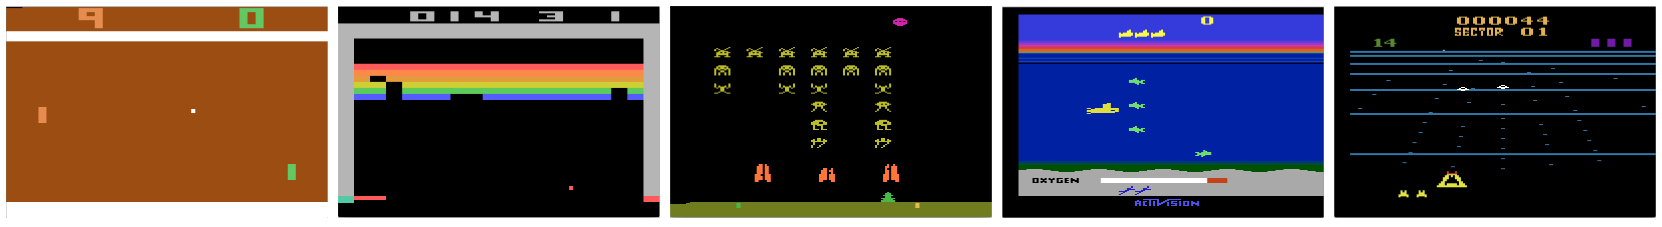
\includegraphics[width=\textwidth]{images/GRL.png}
    \caption{Reinforcement Learning Playing Atari Games \cite{mnih2013playing}.}
    \label{fig:GRL}
\end{figure}

\begin{figure}[h!]
    \centering
    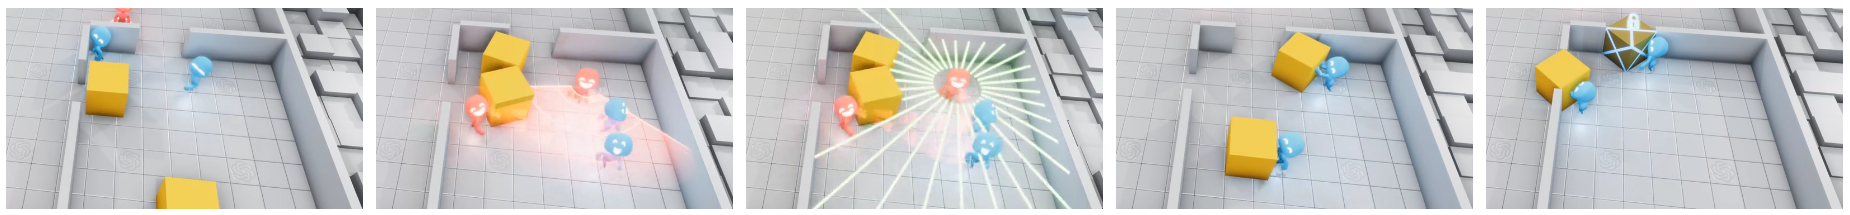
\includegraphics[width=\textwidth]{images/MARL.png}
    \caption{Cooperative Multi Agent Reinforcement Learning \cite{baker2020emergent}.}
    \label{fig:MARL}
\end{figure}

\begin{figure}[h!]
    \centering
    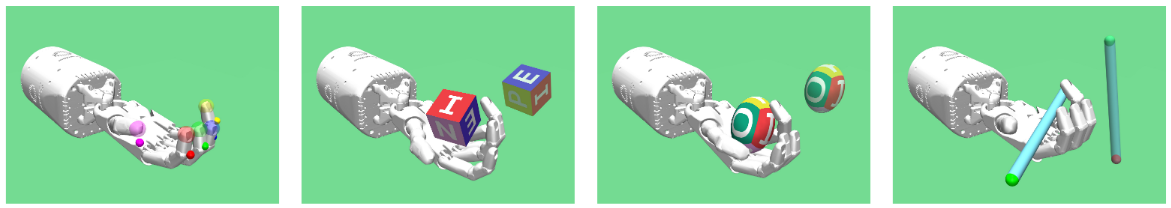
\includegraphics[width=\textwidth]{images/RRL1.png}
    \caption{Dexterous Robotic Manipulations by Reinforcement Learning in Simulation \cite{plappert2018multigoal}.}
    \label{fig:RRL1}
\end{figure}

\begin{figure}[h!]
    \centering
    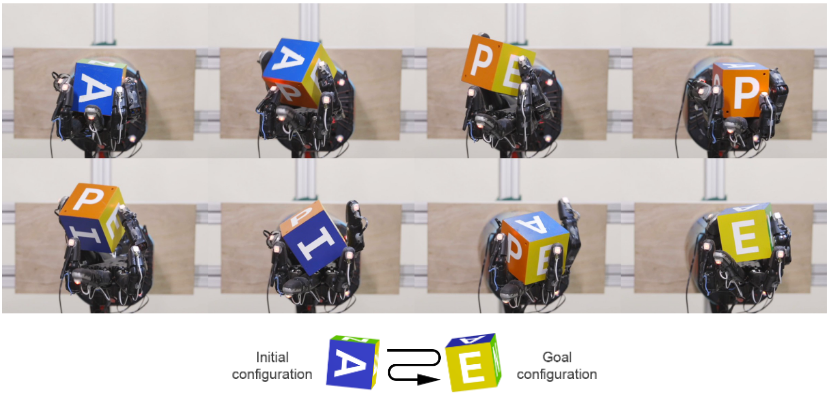
\includegraphics[width=\textwidth]{images/RRL.png}
    \caption{Dexterous Robotic Manipulations by Reinforcement Learning in Real World \cite{openai2019learning}.}
    \label{fig:RRL}
\end{figure}

\begin{figure}[h!]
    \centering
    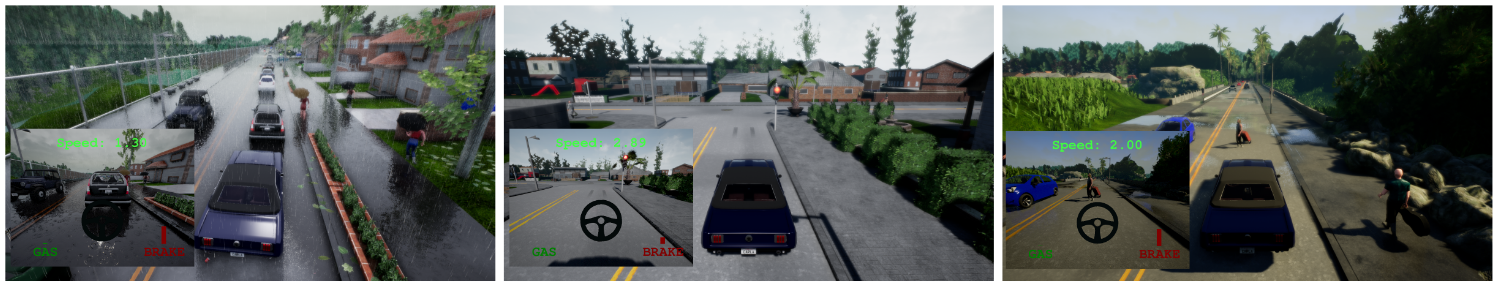
\includegraphics[width=\textwidth]{images/BCAD.png}
    \caption{Behaviour Cloning used for Autonomous Driving \cite{codevilla2019exploring}.}
    \label{fig:BCAD}
\end{figure}

\begin{figure}[h!]
    \centering
    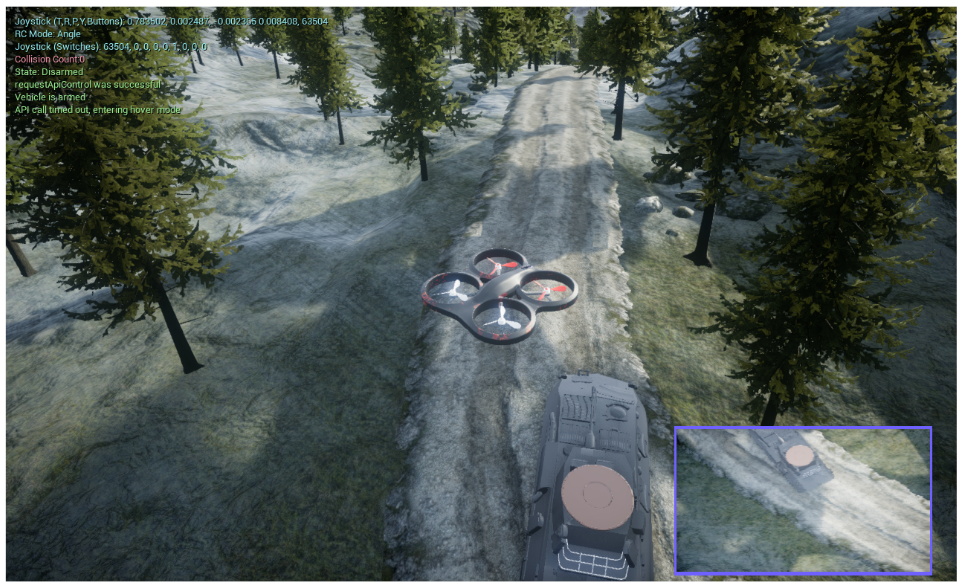
\includegraphics[width=\textwidth]{images/BCRL.png}
    \caption{Behaviour Cloning and Reinforcement Learning used for Drone Landing \cite{goecks2020integrating}.}
    \label{fig:BCRL}
\end{figure}

So what makes it a challenge to apply RL successfully to robotics? One of the main reasons is the nature of the environment itself. Unlike most games where the reward function can be directly optimized to reach the desired objective, robotics tasks are more indirect and goal-based. Most environments in the field of robotics, involve a component like an arm that interacts with an object in the environment to perform tasks like pushing, sliding, picking and placing, etc. Given this scenario a direct reward function alone is not enough to train a policy as the task becomes more goal-oriented, naturally resulting in a case of sparse rewards as seen frequently in newly developed robotics environments. Binary and sparse rewards can be easily defined, for example, positive or zero rewards for completing a task and negative rewards for not completing a task. For robotics-based tasks, this kind of setup is more appropriate than a traditional reward function. Sparse rewards are also easier to work with for a RL agent as it does not get stuck in a local minimum, which is one of the problems that a well-defined dense reward function faces. However, sparse rewards have their own set of unique challenges. The main problem of a sparse reward system compared to a dense reward system is that dense reward provides valuable information for every state the agent visits whereas sparse rewards provide meaningful information only when the agent completes a specific task. Without sufficient information from the reward, a randomly initialized agent with random exploration rarely sees any positive reward signal. The agent becomes sample inefficient and takes exceedingly many interactions with the environment to even see any positive feedback making it slow to converge and taking too long to learn. In some cases, the agent just fails to learn any meaningful actions, in other cases, the agent might end up learning undesirable behaviours which may be acceptable for a simulated environment but may not be suitable for real-world applications. Apart from the concerns of safety and failures, pure offline RL also costs considerable time and hardware resources to train a successful policy. \\

Recent related research \cite{plappert2018multigoal} have been able to successfully implement complex tasks in robotics using RL and sparse rewards. Using different exploration strategies like multi-agent and noise base exploration \cite{lanier2019curiositydriven}. Taking advantage of the off-policy nature of RL algorithms and the experience replay memory trick to overcome these sparse rewards \cite{andrychowicz2018hindsight}. Also, using simulation-based tricks like initializing the environment in a much suitable situation for the agent. In this case, the agent can see a positive reward sooner helping in learning. These and other related researches have found success in RL with sparse rewards but come with a cost in the form of complex and difficult implementations, training time or hardware resources. \\

The key takeaway from this is the need to reduce the training time and accelerate RL in environments with complex dynamics like robotics, with a simple and straightforward implementation, without the need for heavy hardware resources or distributed computing. This is the main motivation behind this research. To achieve this the main area that needs to be addressed is the exploration phase of RL which takes a major chunk of the training time. This time increases with the increase in the state-space, action-space, dynamics and complexity of the environment. \\

One of the approaches to overcome this limitation is to go for a supervised learning approach by using demonstrations sourced from an expert \cite{ARGALL2009469} \cite{RLFD} either in the form of imitation learning \cite{reddy2019sqil} \cite{ILRL} \cite{luo2021selfimitation} \cite{luo2020selfimitation} or transfer learning \cite{Taylor2009TransferLF} \cite{TLMARLS} \cite{zhu2021transfer} \cite{ILTLRL}. Learning from Demonstrations or Behaviour Cloning (BC) is a subset of imitation learning where demonstrations in the form of (state, action) tuple pair from an expert demonstrator are used as a form of supervised learning to induce the desired behaviour and overcome random exploration resulting in higher performance than a randomly initialized agent. Behaviour Cloning learns the mapping of the state-action pairs in the demo dataset and tries to mimic similar behaviour to solve similar tasks. But, plain BC is restricted by the source, quality and quantity of the demonstrations. BC has shown great success \cite{BCAD} \cite{sumanth2020enhanced}, Figure \ref{fig:BCAD} shows the application of behavior cloning for a self-driving car. However, in more complex environments Behaviour Cloning is sometimes known to fail and result in undesirable behaviours. The reason for this is the limited number of demonstrations. Behaviour Cloning takes advantage of demonstrations to solve tasks, but these demonstrations cannot be provided for each and every scenario, and this becomes increasingly difficult as the complexity of the task and environment increases. Also, Behaviour Cloning suffers from a problem called the distributional drift problem, which is the difference in the distribution of the states of the learned policy and the distribution of the states of the expert policy in the demonstrations dataset causing errors that propagate over time resulting in catastrophic failures \cite{goecks2020integrating} \cite{codevilla2019exploring}. One way to solve these problems would be to combine Behaviour Cloning with Reinforcement Learning, which in a sense complement each other by overcoming the other's limitations resulting in a more capable, safer and desirable policy acceptable in simulation and also suitable for real-world applications \cite{gao2019reinforcement} \cite{nair2018overcoming} \cite{vecerik2018leveraging}. Figure \ref{fig:BCRL} shows the combination of Behaviour Cloning and Reinforcement Learning of a drone landing the Microsoft AirSim environment \cite{shah2017airsim}. \\

Another approach in accelerating Reinforcement Learning and overcoming exploration is the reward function. Environments with sparse rewards do not provide enough information for the agent to explore properly and learn successfully. A randomly initialized agent with random exploration takes very long to get positive feedback increasing the training time overall. An over-engineered or well-defined reward function can result in sub-optimal policies, hence the design of the reward function must be done with utmost care. Previous research \cite{nagpal2020reward} \cite{Dewey2014ReinforcementLA} \cite{Konidaris2006AutonomousSK} have shown success in this area for complex environments and was enough motivation to pursue that direction as well in this research to develop a simple yet informative reward function in addition to the combination of Behaviour Cloning and Reinforcement Learning methods mentioned above. \\

The contributions of this research paper are threefold. Firstly, this paper investigates the combination of Behaviour Cloning and Reinforcement Learning with the most recent advances in the respective fields, by proposing a new loss function to combine the Behaviour Cloning Imitation Learning Loss \cite{goecks2020integrating} \cite{nair2018overcoming} with the Actor-Critic based loss function \cite{lillicrap2019continuous} \cite{fujimoto2018addressing} of the Reinforcement Learning agent to accelerate the training. Secondly, this paper proposes a simple yet informative reward function to further aid the Reinforcement Learning agent in training. Thirdly, a training strategy to efficiently train the Reinforcement Learning agent using both the agent's data collected during exploration and the expert's data already collected as a part of the demonstrations dataset. By effectively using demonstrations from an expert as a part of the training process for a Reinforcement Learning agent, the learning can be accelerated even in complex environments. This proposed method has shown success compared to previous baselines and outperformed them. The agent is pretty robust to the source, quality and quantity of the demonstrations. The agent is not constrained or limited to the demo actions present in the dataset. The agent can develop new behaviours and can also outperform the expert demonstrator. The experiments are conducted and tested on the Open-AI Gym \cite{brockman2016openai} and MuJoCo \cite{MJC} based Fetch Robotics Environments \cite{plappert2018multigoal}. \\

\subsection{Research Questions}

The motivation behind this thesis has been explained in the previous section, the research will be focused on those areas and will be aiming to explore and answer the following themes. \\

\begin{itemize}[leftmargin=0.7in]
    \item[Q1.  ] \textbf{Can the proposed method successfully solve complex robotics tasks?} \\
    
    \item This is this first and foremost and most important question preceding the others, given the complex nature of the goal-based task and the dynamics of robotics environments, it would be essential to see if the proposed method can solve all the test environments successfully. \\

    \item[Q2.  ] \textbf{Does the proposed method achieve accelerated learning without a compromise to generalization or resulting in any undesirable outcomes?} \\
    
    \item This next question goes deep into the heart of this research. The main aim of this paper is the acceleration of Reinforcement Learning, hence this question has to be answered in two parts. The first would be to see if that acceleration is indeed achieved by the proposed method. Second, does this acceleration come at a cost, for example in the form of undesirable behaviours, or loss in generalization? \\
    
    \item[Q3.  ] \textbf{Does the source, quality and quantity of the demonstrations used matter for performance?} \\
    
    \item As this method is dependent on a dataset of demonstrations to provide good learning, it is important to ask if the source of the demonstrations has any impact on the performance? What if the available demo data is noisy? What if only a fewer number of demonstrations are collected? This research aims to explore and answer these related questions. \\

    \item[Q4.  ] \textbf{How does the proposed method compare to previous related baselines?} \\
    
    \item The final question is to gauge the performance of the proposed method by comparing this to previous related research, in terms of implementation, convergence rate, training time and hardware resources. \\
\end{itemize}

\subsection{Thesis Outline}

Chapter 1 presents the introduction section where the reader is eased into the main theme of the research in this paper. Related concepts are introduced and the main motivation behind this research is presented. \\

Chapter 2 goes into detail about the theoretical framework involved in structuring this research. Concepts will be explained in more detail and related research will be explored that have directly or indirectly influenced this research. \\

Chapter 3 will look at the proposed methodology in detail, the architecture and algorithm involved in the current research will be explained along with the pseudocode for the framework. Simulators, toolboxes and environments used will be looked at in detail along with experiments conducted and hyperparameters used. \\

Chapter 4 examines the results obtained from the experiments and comparisons will take place depending on the various performance criteria all of which will be explained in detail, followed by a discussion that will further explain what was observed and why with appropriate reasoning. \\

Chapter 5 will finish this paper by summarizing the important concepts and focusing on the main contributions of this research, showcasing what was achieved, what went right, what went wrong and what could be done as an extension for future research. \\


\section{Theoretical Framework}

\subsection{Reinforcement Learning}

Reinforcement Learning solves a particular kind of problem where decision-making is sequential, and the goal is long-term, such as game playing, robotics, resource management, or logistics \cite{100PML}. Reinforcement Learning is a computational approach to understanding and automating goal-directed learning and decision-making \cite{Sutton1998}. It is a subset of Machine Learning in which Intelligent Agents/Autonomous Agents take actions in an environment to complete a given task while aiming to maximize a numerical reward. This concept differs from that of Supervised and Unsupervised learning which together form the three paradigms of Machine Learning. Unlike the Supervised and Unsupervised Learning approaches, Reinforcement Learning is a more interactive approach, it does not have a fixed dataset whether it be labelled or unlabeled and rather uses a moving distribution of observations that results from the actions taken by the agent. This can be categorized as a closed-loop problem as the current actions influence the later inputs as this process repeats \cite{Sutton1998}. \\

\begin{figure}[h!]
    \centering
    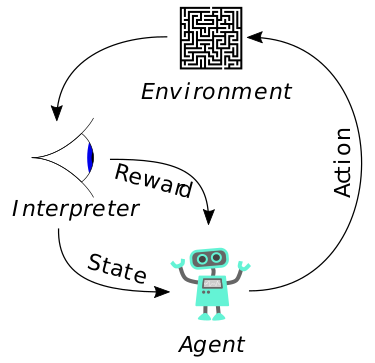
\includegraphics{images/Reinforcement_learning_diagram.svg.png}
    \caption{A simple Reinforcement Learning Scene \cite{wiki}.}
    \label{fig:RLD}
\end{figure}


\subsection{Components of Reinforcement Learning}

Figure \ref{fig:RLD} represents a simple scenario in Reinforcement Learning, where an Agent, which is tasked with achieving a goal in the given environment. The agent accomplishes this task by receiving observations from the environment and interacting with the environment by taking actions and receiving feedback from the environment for the actions taken. In the case of simple environments, the goal can be written directly in terms of a reward function that provide feedback to the agent for each state visited and each action taken, the agent tries to maximize this numerical reward by taking relevant actions and solving the task in the process. The agent here is known as the policy function, which maps the state-action pairs, and for a given state decides which action is appropriate that maximizes the reward. This state-action pair mapping can also be called the value function which determines the quality of the actions taken based on the feedback from the reward function. The aim here is to choose the best action for the given state to receive the highest possible reward. The policy function, value function, and reward function form the three main components of a Reinforcement Learning process that co-exist in a closed-loop system. This system can be modelled as a Markov Decision Process (MDP) \cite{Sutton1998} \cite{FMDP}, which is a discrete time based mathematical framework for modelling sequential decision making. This can be used to solve optimization problems by dynamic programming \cite{DPBE}. Sometimes Reinforcement Learning can include an extra element known as the Model of the environment. This is mentioned here as this too forms an integral part of certain categories of Reinforcement Learning but will not be elaborated in detail as it is out of scope for this research. This research is based on the Model-Free category of Reinforcement Learning. \\

\begin{figure}[h!]
    \centering
    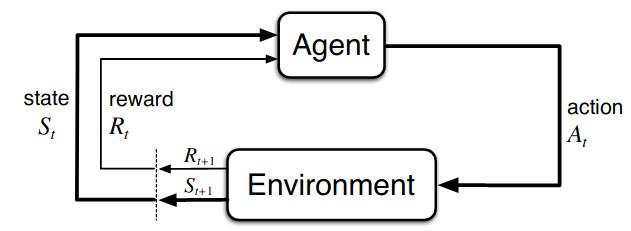
\includegraphics[width=\textwidth]{images/HMM.png}
    \caption{An agent interacting with the environment \cite{Sutton1998}.}
    \label{fig:HMM}
\end{figure}

The agent also known as the policy, usually denoted by $\pi$, is the decision-maker which means it specifies what action $A_t$ to take given a state $S_t$ at time $t$. More precisely $\pi$ gives the probability of an action or a probability distribution for different actions from which the best possible action for the given state is made. These actions are selected based on the reward it receives and the aim is to maximize this return. The expected return $G_t$ at given time $t$ can be formalized as per \ref{eq:1}. The environment here can either be episodic with a fixed number of time steps and a terminal state indicating the end of an episode, or continual which do not have any terminal state and never end. \\

\begin{equation}\label{eq:1}
    G_t = R_{t+1} + R_{t+2} + R_{t+3} + ... + R_T
\end{equation}

In these environments where the $T$ tends to infinity an additional term $\gamma$ also known as the discount factor is added to the above equation to induce simplicity and to prevent the expected returns from reaching infinity. Rewriting the expected returns including the discount factor results in equation \ref{eq:2}. \\

\begin{equation}\label{eq:2}
    G_t = R_{t+1} + \gamma R_{t+2} + \gamma^{2} R_{t+3} + ... + \sum_{k=0}^{\infty} \gamma^{k} R_{t+k+1}
\end{equation}

This discount factor usually has a value between 0 and 1, in most cases, this value tends to be closer to 1. \\

\subsection{V-Function \textit{vs} Q-Function}

The V-Function or state-value function, sometimes known as just Value Function, or simply $V$. This can be defined as the measurement of goodness for an agent to be in a particular state $S_t$ based on the returns $G_t$ following the current policy $\pi$. The value function is the expected total returns which can be discounted or undiscounted and can be expressed with equation \ref{eq:3}. \\

\begin{equation}\label{eq:3}
    V_{\pi} (s) = E_{\pi} [\sum_{k=0}^{T} \gamma^{k} R_{t+k+1} | s=s_t]
\end{equation}

Unlike the value function which defines a value for only the state, the Q-Function or action-value function, or simply $Q$, defines a value for each state-action pair. It can be quantified as a value of taking an action $A_t$ given a state $S_t$ at time $t$ following a policy $\pi$. The Q function can be written as $Q_{\pi} (s, a)$ and is the expected Return $G_t$ starting from $S_0$, after taking an action $A_0$, and then following a policy $\pi$ which can be expressed with equation \ref{eq:4}. \\

\begin{equation}\label{eq:4}
    Q_{\pi} (s, a) = E_{\pi} [\sum_{k=0}^{T} \gamma^{k} R_{t+k+1} | s=s_t, a=a_t]
\end{equation}

\subsection{Bellman Equation $\&$ Optimal Policy}

The Bellman Equation \cite{DPBE} \cite{BE} can be seen extensively in Reinforcement Learning related literature. The Bellman Equation expresses the relationship between the value of a state and the value of the successor states \cite{Sutton1998}. This can be broken down into two essential components the immediate reward and the discounted future rewards. In mathematical terms, the Bellman Equation can be defined by equation \ref{eq:5}. \\

\begin{equation}\label{eq:5}
    V(s) = E [R_{t+1} + \gamma V(S_{t+1}) | S_t = s]
\end{equation}

Based on this general form of the Bellman Equation it can be rewritten to suit both the V-Function and Q-Function as shown by equations \ref{eq:6} and \ref{eq:7}. These equations express the relationship between the value of the state and the value of its successor states. \\

\begin{equation}\label{eq:6}
    V_{\pi}(s) = \sum_{a} \pi (a|s)\sum_{s^{'}} P(s^{'}|s) [R(s, a) + \gamma V_{\pi} (s^{'})]
\end{equation}

\begin{equation}\label{eq:7}
    Q_{\pi} (s, a) = \sum_{s^{'}} P(s^{'}|s, a)[R(s, a) + \gamma\sum_{a^{'}} \pi (a^{'}|s^{'}) * Q_{\pi} (s^{'}, a^{'})] 
\end{equation}

Any policy which can maximize a total cumulative reward can be classified as an optimal policy, represented as $\pi *$. For Finite Markov Decision Processes, an optimal policy exists but may not be unique, meaning there could be different optimal policies sharing a common value function known as optimum value function which can be defined as the function which yields the maximum value, represented by equation \ref{eq:8}. Similar is the case for an optimal action-value function, represented by equation \ref{eq:9}. \\

\begin{equation}\label{eq:8}
    V_{*} (s) = max_{\pi} V_{\pi} (s) 
\end{equation}

\begin{equation}\label{eq:9}
    Q_{*} (s, a) = max_{\pi} Q_{\pi} (s, a)
\end{equation}

Equation \ref{eq:8} and \ref{eq:9} represents the optimal state value function and action-value function which can be further combined with the Bellman Equation to get the Bellman Equation of Optimality as shown by equation \ref{eq:10} and \ref{eq:11} for the state value function and the action-value function respectively. Bellman optimality equation expresses the fact that the value of a state under an optimal policy must equal the expected return for the best action from that state \cite{Sutton1998}. \\

\begin{equation}\label{eq:10}
    V_{*} (s) = max_{a} \sum_{s^{'}} P(s^{'}|s)[R(s, a) + \gamma V_{*} (s^{'})]
\end{equation}

\begin{equation}\label{eq:11}
    Q_{*} (s, a) = \sum_{s^{'}} P(s^{'}|s, a)[R(s, a) + \gamma max_{a^{'}} Q_{*} (s^{'}, a^{'})]
\end{equation}

\subsection{On-Policy \textit{vs} Off-Policy}

The main objective of both types of learning is to evaluate a Q-function $Q(s, a)$ to predict cumulative future discounted rewards given a state $S$ and action $A$. \\ 

In on-policy learning, the $Q(s,a)$ function is learned from actions that are taken using the current policy $\pi(a|s)$. An example of on-policy learning is the SARSA algorithm \cite{zou2019finitesample}. The update rule for the SARSA algorithm as per the Bellman Equation can be written as per equation \ref{eq:12}, where the action $a^{'}$ is taken as per current policy $\pi$. \\

\begin{equation}\label{eq:12}
    Q(s, a) = Q(s, a) + \alpha [r + \gamma Q(s^{'}, a^{'}) - Q(s, a)]
\end{equation}

Comparing this to the off-policy learning, $Q(s, a)$ function is learned from taking different actions including random actions without even the need to define a policy. An example of off-policy learning is the Q-Learning algorithm \cite{QL} where an optimal policy can be reached using random actions for exploration without specifying a policy before learning. The update rule for the Q-learning algorithm as per the Bellman Equation can be written as per equation \ref{eq:13}, where $a^{'}$ are all the actions that were taken in-state $s^{'}$. \\

\begin{equation}\label{eq:13}
    Q(s, a) = Q(s, a) + \alpha [r + \gamma max_{a^{'}} Q(s^{'}, a^{'}) - Q(s, a)]
\end{equation}

The research in this paper is based on the off-policy style of learning algorithms and the related concepts will be briefed in the following sections. \\

\subsection{Q-Learning}

\begin{figure}[h!]
    \centering
    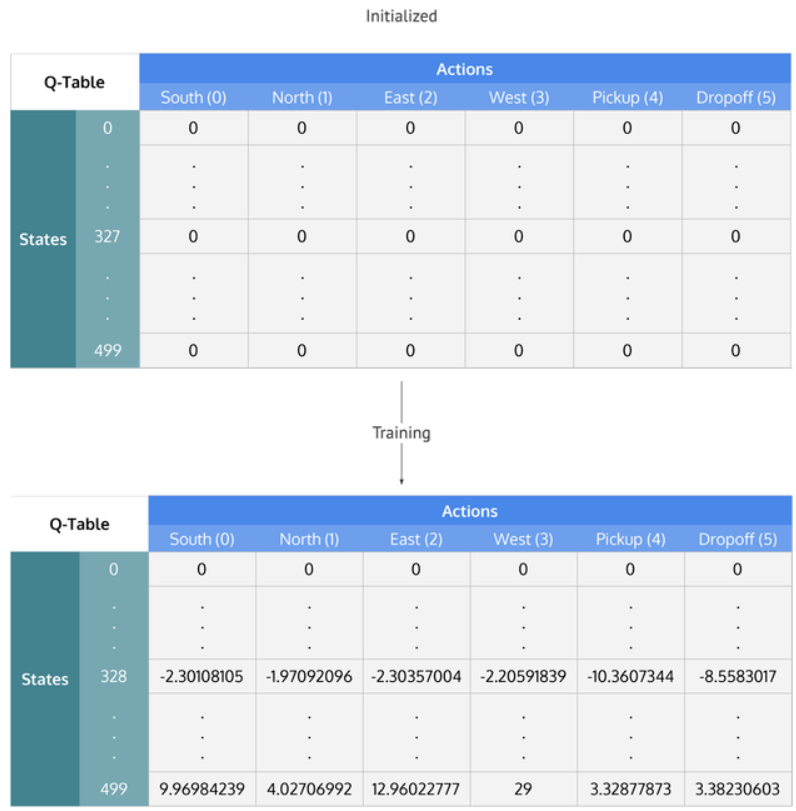
\includegraphics[width=\textwidth]{images/Q-Table.png}
    \caption{A simple example of a Q-Table \cite{wiki}.}
    \label{fig:QT}
\end{figure}

The Q-Learning algorithm \cite{QL} was one of the earliest Reinforcement Learning algorithms proposed in 1989, which even to date is being used in some form. Equation \ref{eq:13} shows the Bellman update rule for the algorithm, where $\alpha$ is the learning rate that controls the convergence rate. The learning rate usually has a value between 0 and 1. \\

Q-Learning is an off-policy Reinforcement Learning algorithm that evaluates an action-value function Q(s, a) to find the optimal action-value function $Q^{*}$. Q-Learning uses a table-based storage system known as Q-Table to store and later look up the Q values for each state-action pair. As the agent explores the environment and makes actions, the Q values are determined using the update equation, and the combination of (Q-value, State, Action) are stored in the Q-Table. Each pair combination of the state and action will have a corresponding Q-value and will be constantly updated using the update rule. Figure \ref{fig:QT} shows a simple Q-Table containing 6 actions and 500 states and the corresponding Q-value for each state-action pair. \\

The Q-Learning algorithm has shown great success by solving many tasks in Reinforcement Learning. But this kind of brute force method has a severe problem. For example in cases where the state space and action space are orders of magnitude higher, storing each and every value and then dynamically searching and updating increases the computation time and hardware resources making this computationally too expensive for simpler tasks. Here is where the generalization capabilities of Artificial Neural Networks \cite{mcculloch1943logical} can be leveraged, instead of storing and updating each and every Q-value, given the state as the input the Q-value can be approximated by a neural network for the set of actions, from which the best action for a given state can be selected. \\

\subsection{Neural Network Function Approximation $\&$ Deep Q-Learning}

\begin{figure}[h!]
    \centering
    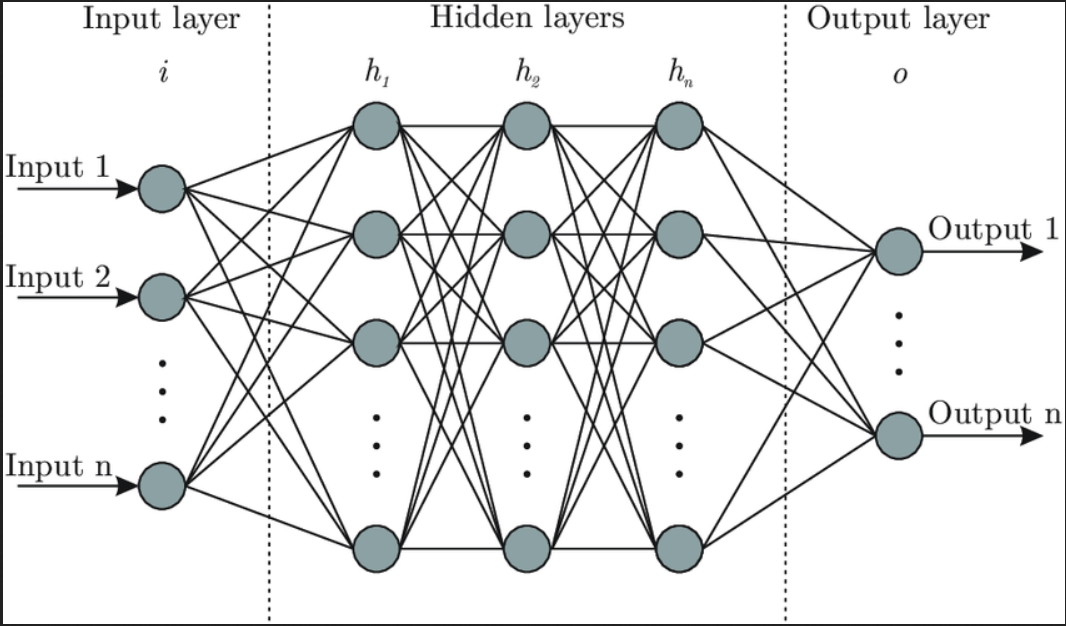
\includegraphics[width=\textwidth]{images/ANN.png}
    \caption{A simple representation of a Neural Network \cite{ANNPic}.}
    \label{fig:ANN}
\end{figure}

Figure \ref{fig:ANN} shows a pictorial representation of a simple Artificial Neural Network (ANN) also known as a Multi-Layer Perceptron in technical terms, derived and developed from the original Rosenblatt Perceptron Model \cite{rosenblatt1958perceptron}. Extensive research has been conducted in this field of deep learning by the likes of Geoffrey Hinton, Yoshua Bengio, Yann LeCun, Ian Goodfellow, Andrew Ng and this research follows and refers to such works. These researchers have covered topics on this field extensively and it will not be detailed elaborately here as it is out of scope for this research. However, basic related concepts will be briefed. \\

The general theory behind a perceptron is, N amount of features is connected to the M amount of outputs with the help of W amount of weights and the strength of these weights between these connections determines the relation between the input and output. In this manner, the input can be mapped to the output by changing or updating the weights. The individual unit in the perceptron is called a neuron, named after the biological neurons present in the nervous system. These neurons take input and after applying a degree of non-linearity give an output, mathematically this can be represented by equation \ref{eq:14}. \\

\begin{equation}\label{eq:14}
    Y_k = \textit{f} [W_{jk} * X_k + B]
\end{equation}

X represents the value of the neuron usually the input, W is the weight of the connection usually initialized with random values, B is a value of bias that is added to every operation and Y is the output after the application of a certain degree of non-linearity. The combination of multiple of these perceptron's to form layers, both horizontally and vertically as represented in figure \ref{fig:ANN} is a multi-layered perceptron, but the basic principle remains the same. By updating these weights the relation between a given input and output can be approximated successfully. Most modern neural networks update their weights by using a technique known as backpropagation \cite{kelley1960gradient}, which can be defined as a gradient descent method to minimize a cost or loss function. This loss function can be defined as per the given problem, an example of a simple loss function is shown in equation \ref{eq:15}. \\

\begin{equation}\label{eq:15}
    MSE = \frac{1}{n} \sum_{i}^{n} (Y_i - Y_i^{'})^2
\end{equation}

To minimize this loss function, the weights can be updated using the weight update equation from the stochastic gradient descent \cite{ruder2016overview} to approximate a function. Immediately this can be seen as a much efficient way when compared to storing values in a lookup table for every input-output pair as discussed in the previous section regarding Q-Learning. Deep Q-Learning (DQN) \cite{mnih2013playing} leverages this power of ANN's to efficiently approximate the Q-values for the state-action pairs. The principle of Deep Q-learning remains the same for the most part, but this eliminates the need for a computationally heavy lookup table and instead uses ANN to predict the Q-values for each action, and for a given state the action with the highest Q-value is chosen as the most probable action at that given time step. \\

\subsection{Double Deep Q-Learning}

As per the Mean Squared Bellman Error Equation, there is a Q-value and a Target Q-value, the error between these values is calculated as the output of the loss function which is then used to update the weights of the network using gradient descent. In DQN both the Q-value and the target Q-value are estimated by a single network in many cases resulting in something called overestimation bias. This means that as the training progresses as the same network is used to estimate two moving values based on maximum returns, it sometimes tends to return higher values for the actions which may not be the best possible choice for that given state. \\

To solve this problem a simple trick was set up, instead of one, two networks were proposed leading to the algorithm called Double Deep Q-Learning (DDQN) \cite{vanhasselt2015deep}. Here there are two copies of the same network, the one estimating the Q-value and the other estimating the Q-target. Q-target remains stationary and is updated every few time steps by copying the weights from the first network. This enables more stable updates without the problem of overestimation. \\

\subsection{Actor Critic Methods}

\begin{figure}[h!]
    \centering
    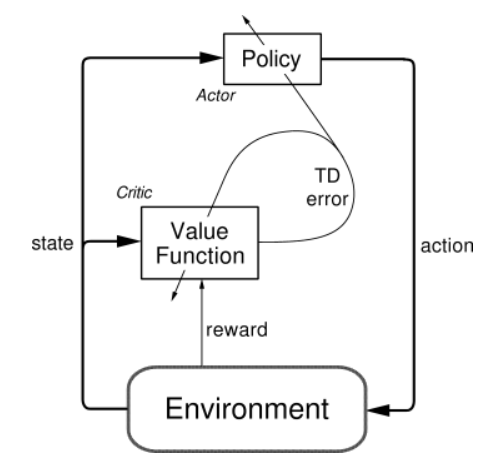
\includegraphics[width=\textwidth]{images/AC.png}
    \caption{Actor Critic Architecture \cite{Konda00actor-criticalgorithms}.}
    \label{fig:AC}
\end{figure}

Policy Gradient \cite{PG} methods are on-policy learning algorithms that target modeling and optimizing a policy directly, unlike Q-learning which does not require a policy to be specified. Temporal Difference \cite{TD} is a technique to predict the expected value given a sequence of states, which acts as a base for most model-free Reinforcement Learning algorithms. Actor-Critic \cite{Konda00actor-criticalgorithms} algorithms are a different class of Reinforcement Learning algorithms but with the same goal which is to find an optimal behaviour strategy that returns maximum rewards.  Simply put Actor-Critic is a Temporal Difference version of Policy Gradient. Another difference between Actor-Critic and Q-Learning is, DQN uses one network to estimate the Q-values of the actions, Actor-Critic use two individual networks one for the Actor and the other for the critic. In DQN for a given state, the network estimates Q-values for all the probable actions, and the action with the highest Q-value is chosen as the best possible action for that given state, in Actor-Critic, the Actor chooses the action for the given state, and the critic evaluates this action by estimating a value function and tells the actor how good the current action is and how to update it further. The actor-network is updated based on the critic value and the critic network is updated by using the actor's actions, both work in tandem and are updated dynamically. This paper will not dive deep into this class of Reinforcement Learning as this is out of scope for this research, but a summary was provided just as an introduction because this is an important concept that will be used as a backbone for other algorithms used extensively in this paper. \\

\subsection{Deep Deterministic Policy Gradients}

DQN style algorithms work well and are more suited for deterministic actions spaces. Deterministic actions spaces have a fixed number of actions, for example, Left, Right, Up, Down. Continuous action spaces as the name suggests have continuous values, for example, any value in the coordinate system. It is not possible to straightforwardly apply Q-learning to continuous action spaces, because in continuous spaces finding the greedy policy requires optimization of actions at every time step, this optimization is too slow to be practical with large, unconstrained function approximators and nontrivial action spaces \cite{lillicrap2019continuous}. A continuous action space can be discretized, but the resulting high number of actions is another limitation that DQN cannot solve. This led to the need for a new class of algorithms able to handle high dimensional continuous action spaces. Research in this area led to a combination of Q-Learning style of learning with the Actor-Critic based algorithms which resulted in the Deterministic class of Reinforcement Learning algorithms of which one of the main algorithms is Deep Deterministic Policy Gradient (DDPG) \cite{lillicrap2019continuous}. \\

DDPG is an off-policy deterministic algorithm which means it returns actions deterministically rather than stochastically \cite{haarnoja2018soft}. The output of a DQN algorithm is probabilistic, which is the highest probability of an action given a particular state, DDPG outputs the exact values of the actions for that given state. DDPG also use an Actor-Critic based architecture, here the actor-network is a policy gradient that takes in states as the inputs and outputs the exact continuous values as actions, the critic-network is a Q-Value network that takes the states and actions as inputs and outputs the corresponding Q-values. The architecture of a DDPG algorithm is designed in such a way that it contains two Actor Networks, a current actor and a target actor, and two Critic Networks, a current critic and a target critic. Both the Current Actor and Critic Networks have their loss functions to minimize during the learning process and the updated weights of the Current Networks are copied onto the target networks. All the four networks are involved during the training process in updating the weights which can be seen from equations \ref{eq:16} and \ref{eq:17}. After the training process is complete only the Actor-Network with the optimal policy can be used for inference. \\

\begin{equation}\label{eq:16}
    J_{Q} = \frac{1}{N} \sum_{i}^{N} [R_i + \gamma (1 - T) Q_{target} (S_{i}^{'}, \mu_{target} (s_{i}^{'})) - Q (s_i, \mu (s_{i}))^2 ]
\end{equation}

\begin{equation}\label{eq:17}
    J_\mu = \frac{1}{N} \sum_{i}^{N} Q(s_i, \mu(s_i ))
\end{equation}

Equation \ref{eq:16} is the critic networks loss function for estimating the Q-values. This loss is very similar to the mean squared bellman loss and it uses both the advancements from the DQN and DDQN algorithms. Here is where the current and target networks come into play in the DDPG algorithm. The current network estimates Q-values for the current states and actions, whereas the target network estimates the Q-values for the next states and the target actions, these target actions coming from the actor target predictions. Equation \ref{eq:17} is the Actor loss which is simply the sum of all the Q-values which the goal is to maximize the result so as the have higher Q-values. Compared to DDQN which performs a hard update by directly copying the weights of the main network to the target network, the new changes introduced here are to perform a soft update instead. Due to dynamic updates and moving Q-values, this provides further stability during the updates which results in faster convergence for the algorithm even in complex environments. The update equations for the target networks are given by Equation \ref{eq:18} and \ref{eq:19}. \\

\begin{equation}\label{eq:18}
    \theta^\mu_{target} = \tau \theta^\mu_{target} + (1 - \tau)\theta^\mu
\end{equation}

\begin{equation}\label{eq:19}
    \theta^Q_{target} = \tau \theta^Q_{target} + (1 - \tau)\theta^Q
\end{equation}

Here $\tau$ is the parameter that controls the degree to which the parameters are copied during the soft update, this value usually lies between 0 and 1, and is typically chosen closer to 1. \\

\subsection{Twin Delayed Deep Deterministic Policy Gradients}

DDPG has shown great success in many complex tasks and even solving robotics tasks which is the essence of this research. It has also been used as the base algorithm for many other successful related research. While it can achieve great performance it can also be brittle sometimes concerning hyperparameters and takes longer to converge, resulting in higher training and tuning times. One of the main failures of DDPG is the Q-Network's overestimation of the Q-values. This overestimation leads to the higher Q-values for actions that may not be suitable for the given state, and when the actor learns from these Q-values the policy beings to break or diverge to some unsuitable behaviour. \\

To fix these issues and improve the performance of the baseline DDPG algorithm, a new method called the Twin Delayed Deep Deterministic Policy Gradients (TD3) \cite{fujimoto2018addressing} was proposed. TD3 aims to address a few of the shortcomings of DDPG by using three new implementations. First, Clipped Double Q-Learning, TD3 uses two Q-Networks unlike DDPG which uses one and uses the smaller of the two estimated Q-values in the mean squared bellman equation, this is a simple and intuitive method of reducing the overestimation bias of the Q-values. Second, Delayed Policy and Target updates, along with the soft update rule the TD3 algorithm updates both the Actor Networks and the target networks in a delayed manner. As per the paper, the Actor and the Target Networks are updated once every two Q-Network updates. This manner of updates allows the actor to see better Q-values along with improved stability leading to robust learning and faster convergence. Third, Target Policy Smoothing, TD3 adds some noise to the target actions, which is the output of the target actor-network, this is to make it harder for the policy to exploit Q-function errors by smoothing out Q-values \cite{fujimoto2018addressing}. Together these improvements result in sustained and improved performance, better stability and faster convergence when compared to DDPG and TD3 will be used and the base algorithm in this research. \\

\subsection{Experience Replay Memory}

The involvement of neural networks in combination with off-policy Reinforcement Learning has shown great success and one of the important reasons is the use of Experience Replay \cite{zhang2018deeper} \cite{fedus2020revisiting}. This is a simple method that enables the agent to save data as it interacts with the environment. The usual format of saving data is $(S_t, A_t, R_{t+1}, S_{t+1})$, Current State, Current Action, Reward, Next State. The recent versions of the experience replays include an additional term that specifies the end of an episode known as the terminal state. This flag is useful in determining whether or not to calculate the discounted future rewards. The data is stored in this format in the memory continuously on a first in first out basis. For learning the agent can randomly sample a mini-batch from the memory and use this to update its weights. This random sampling of a mini-batch from the memory is highly advantageous by introducing a degree of variance as consecutive examples in a Reinforcement Learning environment are highly temporally correlated, and gradient descent methods do not perform well with correlated data. \\

There have been many recent advances with experience replay, namely Prioritized Experience Replay (PER) \cite{schaul2016prioritized} which changes the way how data is presented to the agent emphasizing on data with greater TD error which has shown to speed up training, Hindsight Experience Replay (HER) \cite{andrychowicz2018hindsight} taking advantage of the replay memory to augment the data with new rewards in a sparse reward system where the agent does not get to see positive feedback and in the process accelerates training. The research is this paper does not use any advanced version of experience replay and just uses two replay buffers instead which will be explained in detail in the methods section. \\

\subsection{Hindsight Experience Replay}

\begin{figure}[h!]
    \centering
    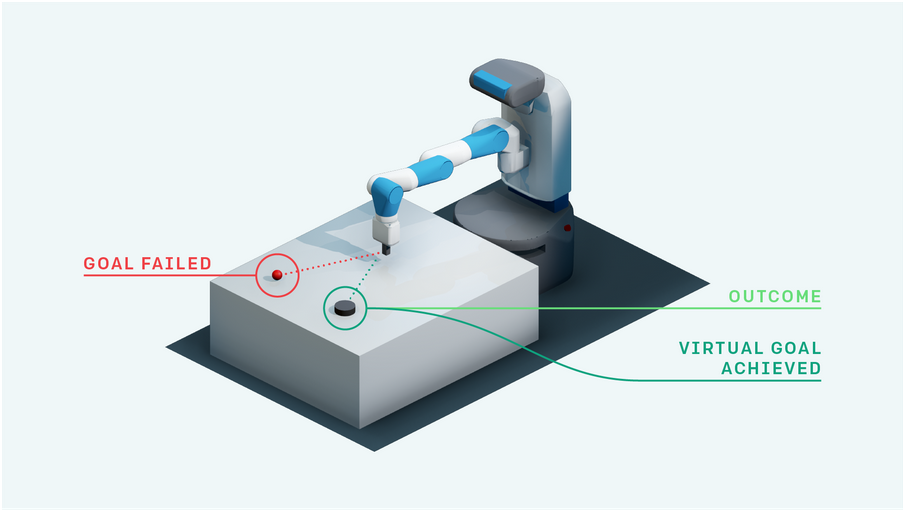
\includegraphics[width=\textwidth]{images/HER.png}
    \caption{Example of Hindsight Experience Replay \cite{andrychowicz2018hindsight} \cite{plappert2018multigoal}.}
    \label{fig:HER}
\end{figure}

HER provides a very intuitive solution by taking advantage of the off-policy replay memory trick by augmenting new data into the already present data in the memory. Such a system is highly useful in environments where the reward is sparse. Sparse reward environments provide almost no information to the agent during the initial phase of learning. Traditionally the agent takes a very long time to see any positive reward hence resulting in large training times. As sparse reward environments are goal-based environments, HER augments the data by providing a positive reward to the achieved goals even though they might be failed instances with the actual goal still to be reached. For example, when the agent in a walking simulator has to reach a particular destination of 100m in the environment but ended up falling short by 20m, the episode has ended and the agent has not reached its main goal. But, what HER does here is it uses the already reached goal of 80m and other similar instances and provides it with a positive reward, the original reward from the environment being negative. By providing positive feedback sooner in the form of virtual goals the agent can see more rewards and in the process eventually end up reaching the desired goal as seen by a simple representation in figure \ref{fig:HER}. This process has shown great success in sparse reward environments and solving complex robotics tasks \cite{plappert2018multigoal}. There are different strategies used for such data augmentation like randomly assigning failed instances as virtual goals, using the end of the episode as virtual goals, or using a distance-based method \cite{HERER} to assign virtual goals to achieve the original goal faster, further accelerating the training in such environments. \\

\subsection{Exploration Exploitation Dilemma}

\begin{figure}[h!]
    \centering
    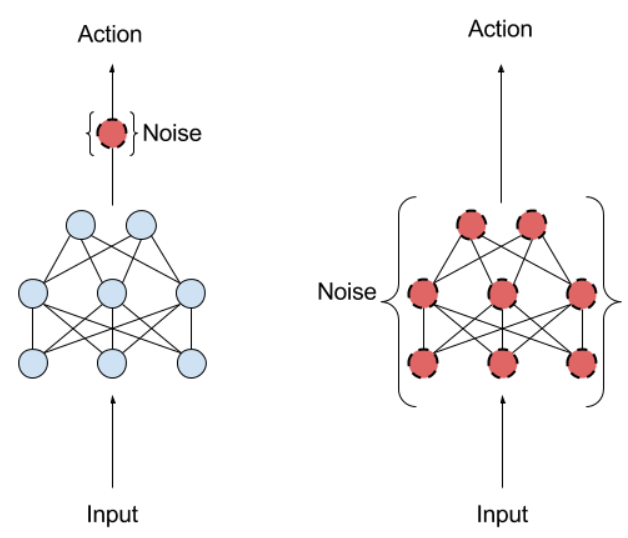
\includegraphics[width=\textwidth]{images/ANPN.png}
    \caption{Difference Between Action Noise and Parameter Noise \cite{plappert2018parameter}.}
    \label{fig:ANPN}
\end{figure}

All Reinforcement Learning algorithms have to go through two important phases during the training process, the exploration phase and the exploitation phase. To maximize the returns the agent needs to learn from the past actions which were desirable and repeat those actions to increase the cumulative reward, this process is known as exploitation. But, to select the best actions the agent needs to perform different actions and receive feedback from the environment to determine which of these actions are the best. The trade-off between exploration and exploitation is known as The Exploration-Exploitation Dilemma which has been an active area of research in Reinforcement Learning for many years. \\

One fairly common approach is called the Epsilon-Greedy or $\epsilon$-Greedy Strategy. In this strategy, the agent starts by taking random actions to explore the different states. The $\epsilon$ parameter controls the degree to which the agent takes random or greedy actions. Actions from the agent are known as greedy actions. Over the course of training the $\epsilon$ starts which a high value making the agent take random actions and then the value of $\epsilon$ is reduced and the agent transitions from taking random actions to greedy actions. This way the agent first starts with exploring the environment then goes to exploiting in the later stages of training and a balance between exploration and exploitation is achieved. The $\epsilon$ value is not made entirely zero as even during the exploitation phase some amount of random exploration is desired, and the rate of decrement of this $\epsilon$ value can be controlled as per requirement. \\

This strategy is highly used in Q-Learning related algorithms. The more deterministic algorithms like DDPG and TD3 use noise-based exploration strategies. Noise is induced in some form associated with the actions and this way the agent explores the environment. The network is trained with the noise and learns this noise during the exploitation phase resulting in more robust policies. Two types of noise can be added as seen in figure \ref{fig:ANPN}, one is the action noise \cite{lillicrap2019continuous} \cite{fujimoto2018addressing}, where the noise is directly added to the output actions of the actor-network, the second is the parameter noise \cite{plappert2018parameter}, where noise is added to the weights of the actor-network resulting in perturbed actions. \\

Exploration is an important part of Reinforcement Learning as, without exploration, exploitation is not possible and also does not make sense. For complex environments like robotics, the exploration becomes difficult and this phase takes a major part of the training time to explore the high dimensional state spaces to efficiently exploit the good actions. To accelerate Reinforcement Learning some strategies need to be used to overcome this exploration phase like curiosity-driven exploration with intrinsic rewards \cite{burda2018exploration}, multi-agent exploration \cite{lowe2020multiagent}, the combination of both \cite{lanier2019curiositydriven}, or by leveraging the power of demonstrations which is an important area of focus for this research. \\

\subsection{Reward Engineering}

\begin{figure}[h!]
    \centering
    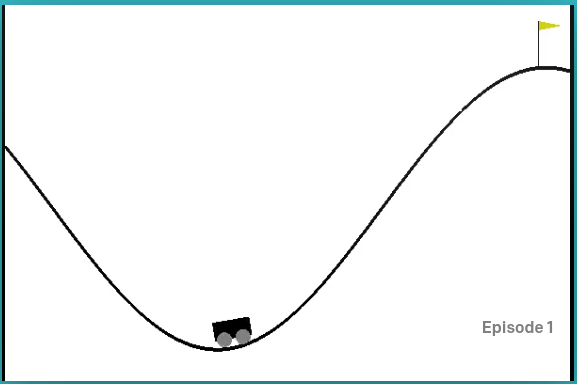
\includegraphics[width=\textwidth]{images/MC.png}
    \caption{Open AI Gym Simple Mountain Car Environment \cite{brockman2016openai}. }
    \label{fig:MC}
\end{figure}

A reward function is one of the three basic components of Reinforcement Learning. As mentioned in the earlier parts of the literature a Reinforcement Learning agent aims to maximize the rewards to ultimately reach an optimal policy. This makes the design of the reward function as important as the design of the policy or the algorithm because the reward function has the power to control the training of the agent. Figure \ref{fig:MC} shows the example of a simple mountain car environment where the reward can be designed in terms of the distance to the flag and velocity of the vehicle as well, but a simple distance reward will do well in this case. A Reinforcement Learning algorithm can directly optimize this reward to reach a good policy. In complex environments which high dynamics such as robotics, a straightforward metric based reward function is not possible due to the involvement of complex interactions. This raises a need for research into reward design for complex environments. The trade-off here is, a simple reward design may not be as effective in enabling the agent in reaching an optimal solution, while a well-engineered reward function may lead to sub-optimal policies. The reward function also plays a major role in the exploration-exploitation phases of the agent, so there is a need to design an optimal reward function balancing the exploration and exploitation, by providing the correct information to the agent, so that it can learn efficiently. Previous research "Reward Engineering for Object Pick and Place Training" \cite{nagpal2020reward} has found success in this area of reward engineering for complex robotics tasks and using that as motivation this area will be an important focus for this research. One of the aims of this research is to design a simple and effective reward function that can provide fast and robust learning. \\

\subsection{Imitation Learning $\&$ Behavior Cloning}

The two main areas of research related to decision making in autonomous robots in recent times are Reinforcement Learning and imitation learning. The basic idea of imitation learning, sometimes known as learning from demonstrations, is that the learning agent receives examples on how to perform actions from an expert demonstrator, and the agent mimics these actions to try and replicate the expert's behaviours. Humans widely use a similar form of learning by referring to experts and trying to mimic those actions as well as retrying similar actions themselves to solve a particular task. The main focus of this research is to try and combine both to solve complex tasks. \\

The simplest and most common form of imitation learning among many others is Behaviour Cloning which uses a supervised learning approach to train an agent. There is a dataset of expert demonstrations in the form of state-action pairs and the agent is trained by minimizing a loss function that estimates the error between the agent's actions and the expert's actions for the given states. A simple Behaviour Cloning loss function can be written like equation \ref{eq:20}. \\

\begin{equation}\label{eq:20}
    BC_{loss} = \frac{1}{n} \sum_{i}^{n} (A_{expert} - A_{agent})^2
\end{equation}

Behaviour Cloning has shown success in many areas solving complex tasks like self-driving \cite{bojarski2016end}, drone navigation \cite{QN}, biped locomotion \cite{BL}, but struggles with generalization outside the demonstration data. Plain Behaviour Cloning heavily relies on the quality and quantity of demonstrations and either perform well for certain tasks or other tasks, worse than a random agent sometimes resulting in undesirable behaviours. Several techniques help with data augmentation and expert data but they constantly rely on the expert being present even during training and cannot do with just a pre-collected dataset. \\

\subsection{Behavior Cloning $\&$ Reinforcement Learning}

Some of the drawbacks of Behaviour Cloning can be solved by combining it with Reinforcement Learning. Previous work has been successful in doing so, demonstrations have been used to speed up learning in simple environments such as cart-pole \cite{RLFD}. Recent works have shown great success in this front by managing to solve complex multi-goal robotics tasks \cite{nair2018overcoming}. This research is very closely related to two recent works combining Behaviour Cloning and Reinforcement Learning, "Overcoming Exploration in Reinforcement Learning with Demonstrations" \cite{nair2018overcoming} and "Integrating Behavior Cloning and Reinforcement Learning for Improved Performance in Dense and Sparse Reward Environments" \cite{goecks2020integrating}. This research aims to accelerate Reinforcement Learning for complex multi-goal robotics environments by leveraging demonstrations. Previous research has shown success in the same tasks but it either comes in the form of complex implementations or the use of heavy computing resources. \\

\section{Methods} \label{section:methods}

\subsection{Current Implementation}

The current implementation is a combination of two main areas of research with a motivation to accelerate reinforcement learning. The reinforcement learning algorithm used in this research is the Twin Delayed Deep Deterministic Policy Gradient (TD3) which has shown better performance compared to its widely used predecessor DDPG. The two areas of focus in this research will be, combining behavior cloning with reinforcement learning which is the combination of BC + TD3 and designing an optimal reward function. \\

\subsection{Loss Functions}

\subsection{Q-Filter}

\subsection{Replay Buffer}

\subsection{Demonstrations}

\subsection{Training Strategy}

\subsection{Reward Design}

\subsection{Deep Learning Specifications}

\subsection{Hyperparameters List}

\subsection{Algorithm Pseudocode}

\subsection{Simulation Environments $\&$ Task Description}

\begin{figure}[h!]
    \centering
    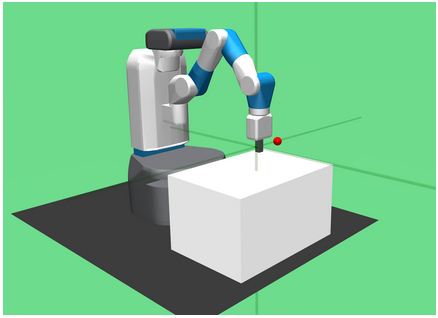
\includegraphics{images/FR.png}
    \caption{Simple Representation of the Fetch Reach Task}
    \label{fig:FR}
\end{figure}

\begin{figure}[h!]
    \centering
    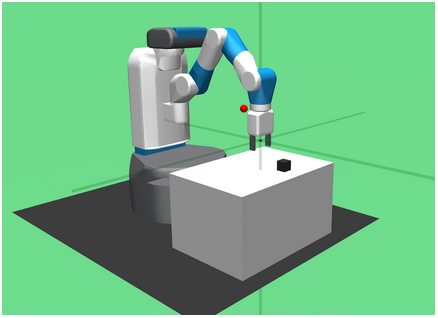
\includegraphics{images/FPAP.png}
    \caption{Simple Representation of the Fetch Pick And Place Task}
    \label{fig:FPAP}
\end{figure}

\begin{figure}[h!]
    \centering
    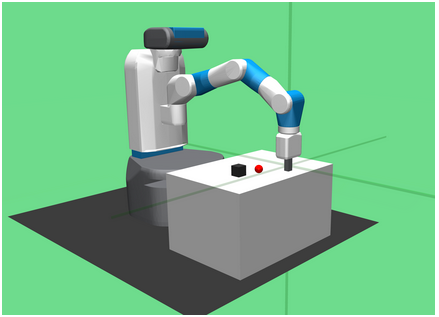
\includegraphics{images/FP.png}
    \caption{Simple Representation of the Fetch Push Task}
    \label{fig:FP}
\end{figure}

\begin{figure}[h!]
    \centering
    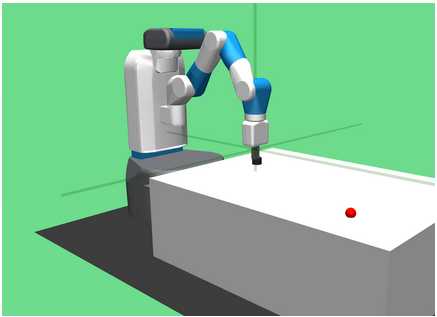
\includegraphics{images/FS.png}
    \caption{Simple Representation of the Fetch Slide Task}
    \label{fig:FS}
\end{figure}

The current implementation





\section{Results}

\subsection{Baselines $\&$ Comparisons}

The first baseline is the combination of reinforcement learning and hindsight experience replay. The combination of DDPG+HER when proposed was able to achieve much success in solving complex multi-goal robotics tasks and has set a benchmark for future research to come. This is an environmental baseline and was the first to solve sparse reward environments used in this research and will be used to compare the current implementation's capability to solve the environment successfully. \\

The second baseline is much closer to this research in terms of algorithm and implementation also combining behavior cloning with reinforcement learning. DDPG+BC along with expert demonstrations was able to successfully accelerate complex robotics tasks in the mentioned environments. This is an algorithmic baseline that was first provided accelerated learning for the environments used in this research and will be used to compare the current implementation's capability to further provide accelerated learning. \\

The third baseline implements pure behavior cloning using demonstrations and will serve as a comparison for why this method has either great or really poor performance. \\

The fourth baseline implements plain reinforcement learning without demonstrations or hindsight experience replay but with dense rewards and was able to achieve good performance in accelerating complex multi-goal robotics tasks. This is a reward baseline that first proposed a new reward function for the multi-goal robotic sparse reward environments used in this research and will be used to compare the current implementation's capability to provide accelerated learning. \\

Apart from comparison with the baselines, there will be other comparisons as well, first with the current implementation itself but with a different demonstration source. The main reason for this comparison is if the current framework implementation is kept fixed while varying different sources of demonstrations, will there be any impact on the performance of the algorithm. Second, there will be a comparison between the generalization capabilities between the current implementation and baseline 1 to check if after the training phase the agent can perform well in the testing phase as well. The third will be a short comparison between the network complexity used between the current implementation and baseline 2 to see if the acceleration comes at a cost of model complexity, also this being very similar approaches the number of demonstrations used will also be compared to see if good performance can be achieved using lesser number of demonstrations. Finally, there will be a comparison between the hardware used and training time for the current implementation and baselines 2, 4 to see if the current implementation can strike a balance between the training time and hardware resources used. \\

The comparison between the current implementation and the baselines will take place in terms of task success rate. The success rate is calculated during the testing phase of the training runs and if the agent can successfully end the episode with a successful task completion then the success rate for that agent is incremented. The baselines calculate the success rate by performing 10 deterministic roll-outs per worker and then calculate the average per test set then averaged across all the workers. One of the main advantages of the current implementation is that it does not require multi-processing or parallel implementations with parallel workers like the baselines and uses just one worker with one roll-out test set from which the average success rate is calculated. The plot represented the average success rate of the test run set during the training phase and the performance will be determined by how soon the agent can achieve the highest possible success rate for a given task. Further comparisons will be in terms of training times vs hardware complexity and model complexity. \\

For task 1 the current implementation will be compared to only baseline 1, baselines 2 and 3 are not available for comparison due to the comparatively simple nature of the environment it was not implemented as a part of this baseline research, but in this paper results for the current implementation is presented for this environment to stay consistent across all the environments in the fetch robotics environment suite. For tasks 2 and 3 the current implementation will be compared with baselines 1, 2 and 3. Baseline 4 will be used only for task 4 as that research only focuses on this particular environment. The comparison between different sources of demonstrations will also be done only for task 4 due to the use of a handcrafted script as a different source of demonstration. This script was not developed as a part of this research and was provided by the baselines team \cite{stable-baselines} as an example for this particular environment. \\

Some abbreviations used in the results to denote the number of time steps are, K and M which corresponds to 1 Thousand and 1 Million respectively. \\

\subsection{Fetch Reach Environment}

\begin{figure}[h!]
     \centering
     \begin{subfigure}[b]{0.4\textwidth}
         \centering
         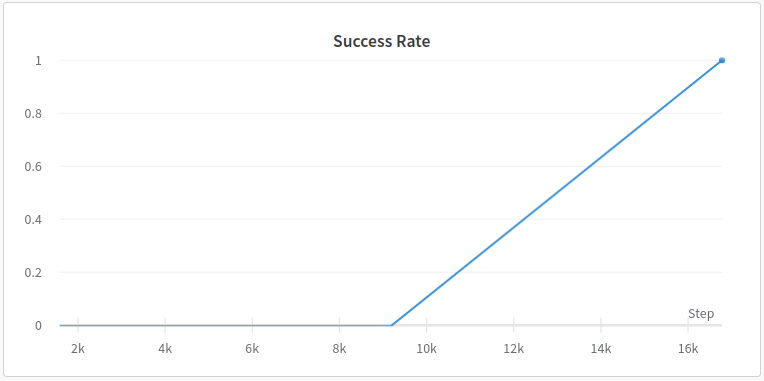
\includegraphics[width=\textwidth]{images/FRSR.png}
         \caption{Success Rate Plot of the Current Implementation.}
     \end{subfigure}
     \begin{subfigure}[b]{0.4\textwidth}
         \centering
         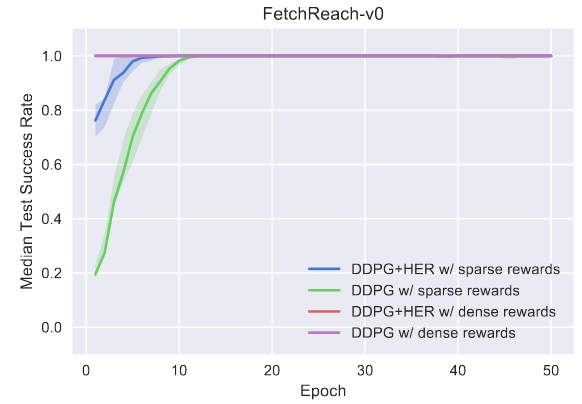
\includegraphics[width=\textwidth]{images/FRB.png}
         \caption{Success Rate Plot for Baseline 1 \cite{andrychowicz2018hindsight}.}
     \end{subfigure}
        \caption{Comparison Between Current Implementation and Baseline 1 for Fetch Reach Task, Epoch Number (every epoch = 800 episodes = 800x50 time steps).}
        \label{fig:FRR}
\end{figure}

In the fetch reach environment, compared to baseline 1, the current implementation has a much higher convergence rate. Figure \ref{fig:FRR} shows the current implementation can reach a success rate of 1.0 at approximately 16K time steps whereas baseline 1 reaches the same success rate of 1.0 at approximately 150K time steps. Not only does the current implementation solve the task successfully but also provides accelerated learning for this environment. \\

\subsection{Fetch Push Environment}

\begin{figure}[h!]
     \centering
     \begin{subfigure}[b]{0.4\textwidth}
         \centering
         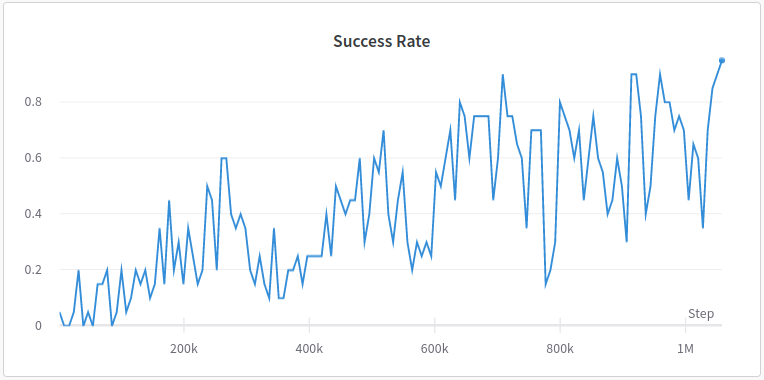
\includegraphics[width=\textwidth]{images/FPSR.png}
         \caption{Success Rate Plot of the Current Implementation.}
     \end{subfigure}
     \begin{subfigure}[b]{0.4\textwidth}
         \centering
         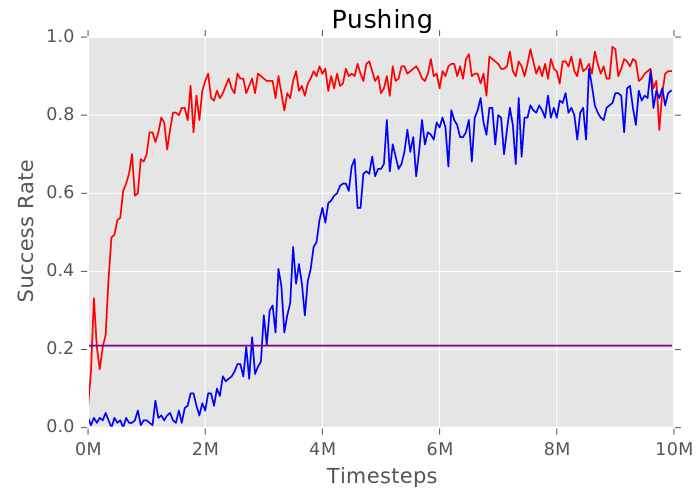
\includegraphics[width=\textwidth]{images/FPB.png}
         \caption{Success Rate Plot for \textcolor{blue}{Baseline 1}, \textcolor{red}{Baseline 2}, \textcolor{violet}{Baseline 3} \cite{nair2018overcoming}.}
     \end{subfigure}
        \caption{Comparison Between Current Implementation and Baselines 1, 2 and 3 for Fetch Push Task.}
        \label{fig:FPR}
\end{figure}

In the fetch push environment, baseline 3 performs the worst by achieving a success rate of only 0.2, performing similar or worse than a random agent. Baseline 1 can successfully solve the environment and reaches a success rate of 0.8 in 10M time steps and baseline 2 can beat it by reaching a success rate of 0.9 in 3M time steps and a success rate of 0.95 in 6M time steps. Figure \ref{fig:FPR} shows that the current implementation can beat all the previous baselines by reaching a success rate of 0.95 in approximately 1.1M time steps, solving the environment successfully and also providing accelerated learning. An interesting observation here is that the demonstrations used had a clear pushing motion where the end effector of the robot arm is used to push the block towards the goal. However, the final agent learned behavior is slightly different from what is expected. The agent can use the end effector of the robot arm to successfully move the object to the goal, but instead of a pushing motion, it uses a poking motion. The main reason could be the dynamics of the environment, MuJoCo uses a soft body collision system for its interactions. This might have influenced the agent to interact differently with the objects in the environment. Even though the goal might be successful, this particular motion might not be a desirable behavior for real-world applications. This can easily be fixed by changing the constraints to rigid body collisions, but this was not done for this research as this process increases the simulation time of the environment significantly. But one positive outcome is that the agent in the current implementation is not bound or constrained to the actions of the demonstrations, it can modify its actions as per the environment and develop new behaviors. As an extension to this research, it would be interesting to try out two things, in the same environment try to use rigid body collisions and then observe the new behavior or try to find a way to overcome the soft body constraints and develop a usable behavior. \\

\subsection{Fetch Slide Environment}

\begin{figure}[h!]
     \centering
     \begin{subfigure}[b]{0.4\textwidth}
         \centering
         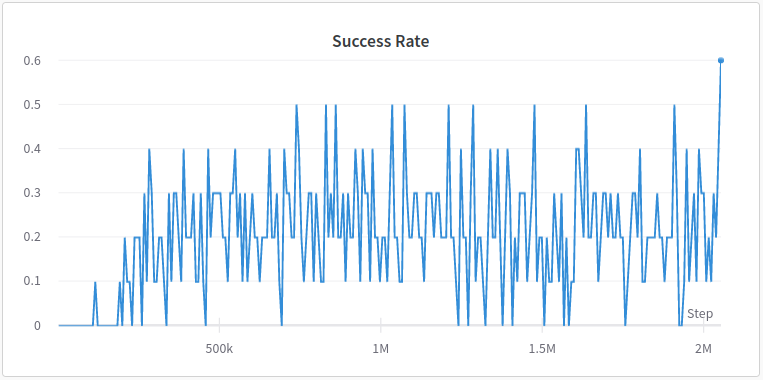
\includegraphics[width=\textwidth]{images/FSSR.png}
         \caption{Success Rate Plot of the Current Implementation.}
     \end{subfigure}
     \begin{subfigure}[b]{0.4\textwidth}
         \centering
         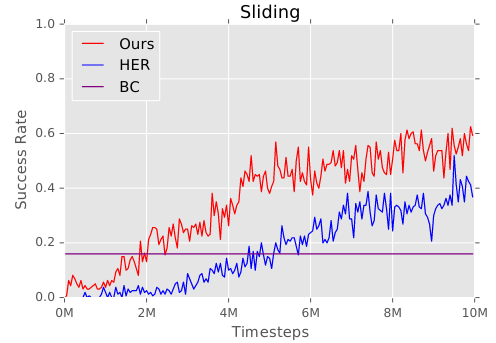
\includegraphics[width=\textwidth]{images/FSB.png}
         \caption{Success Rate Plot for \textcolor{blue}{Baseline 1}, \textcolor{red}{Baseline 2}, \textcolor{violet}{Baseline 3} \cite{nair2018overcoming}.}
     \end{subfigure}
        \caption{Comparison Between Current Implementation and Baselines 1, 2 and 3 for Fetch Slide Task.}
        \label{fig:FSR}
\end{figure}

The fetch slide is the most complex environment of the suite and that is evident by looking at figure \ref{fig:FSR}. Baseline 3 fails this environment as well and achieves a success rate of only 0.2, very similar to the fetch push environment. The baseline 1 can solve the environment but the performance is poor with a success rate of 0.4 in 10M time steps. Both the baseline 2 and current implementation can solve the environment as well and both reach a respectable success rate of 0.6, the baseline 2 can do this in 10M time steps whereas the current implementation can achieve it in just 2M time steps showing a successful acceleration in learning. As an extension to this research, it would be interesting to see whether the current implementation if trained for longer will be able to achieve a higher success rate. \\

\subsection{Fetch Pick and Place Environment}

\begin{figure}[h!]
     \centering
     \begin{subfigure}[b]{0.4\textwidth}
         \centering
         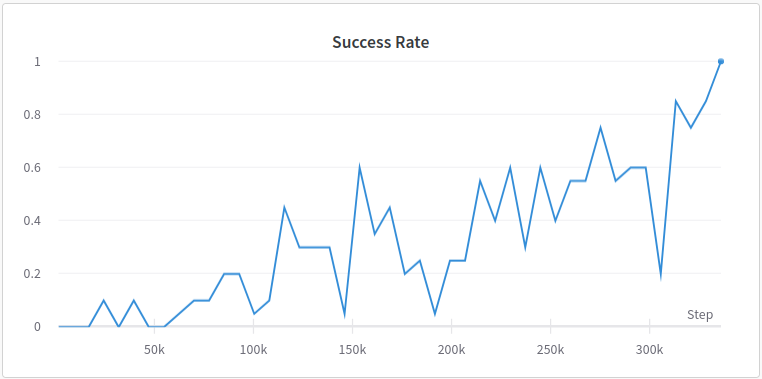
\includegraphics[width=\textwidth]{images/FPAPASR.png}
         \caption{Success Rate Plot of the Current Implementation.}
     \end{subfigure}
     \begin{subfigure}[b]{0.4\textwidth}
         \centering
         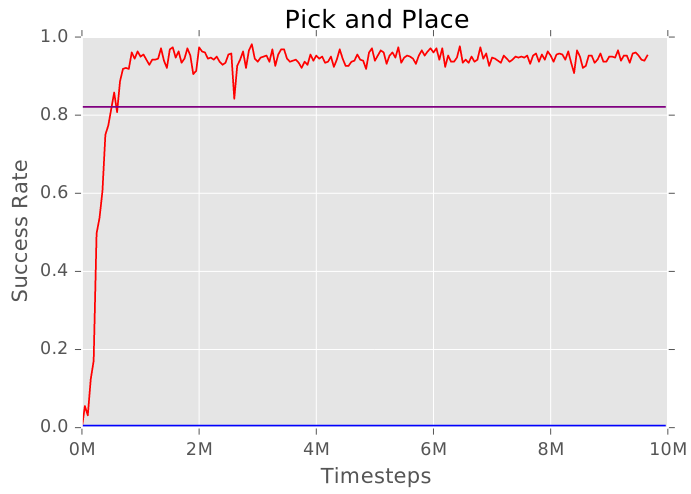
\includegraphics[width=\textwidth]{images/FPAPB.png}
         \caption{Success Rate Plot for \textcolor{blue}{Baseline 1}, \textcolor{red}{Baseline 2}, \textcolor{violet}{Baseline 3} \cite{nair2018overcoming}.}
     \end{subfigure}
        \caption{Comparison Between Current Implementation and Baselines 1, 2 and 3 for Fetch Pick and Place Task.}
        \label{fig:FPAPR1}
\end{figure}

\begin{figure}[h!]
     \centering
     \begin{subfigure}[b]{0.5\textwidth}
         \centering
         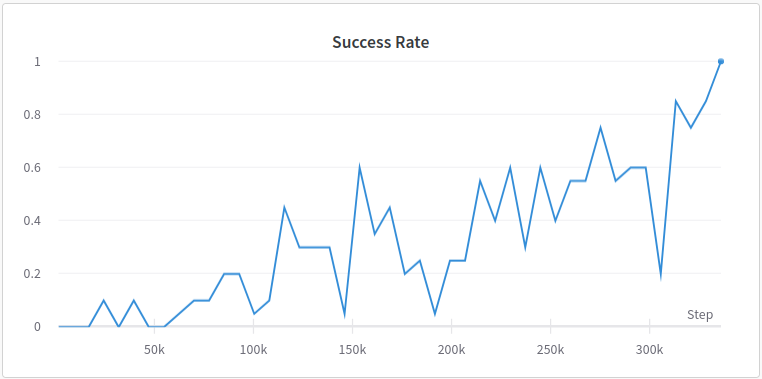
\includegraphics[width=\textwidth]{images/FPAPASR.png}
         \caption{Success Rate Plot of the Current Implementation.}
     \end{subfigure}
     \begin{subfigure}[b]{0.5\textwidth}
         \centering
         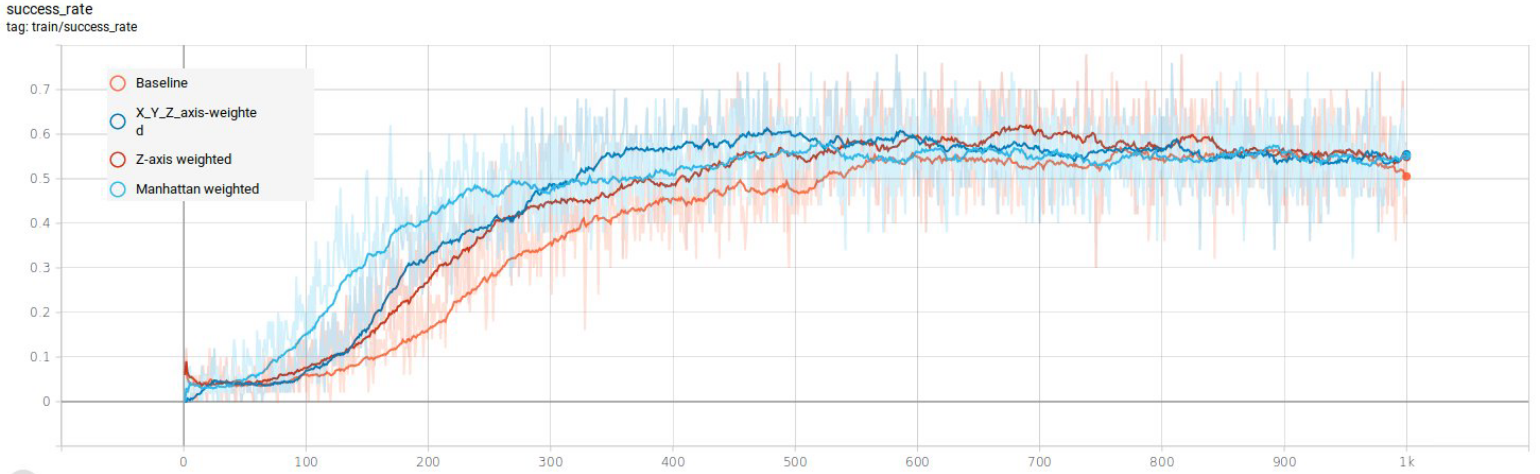
\includegraphics[width=\textwidth]{images/FPAPRRE.png}
         \caption{Success Rate Plot for Baseline 4 \cite{nagpal2020reward}.}
     \end{subfigure}
        \caption{Comparison Between Current Implementation and Baseline 4 for Fetch Pick and Place Task.}
        \label{fig:FPAPR2}
\end{figure}

The fetch reach environment is not as difficult compared to the fetch slide but presents its unique challenges as it involves complex interactions with the object and the gripper. Baseline 3 showing poor performance in the other environments does well in this task achieving a success rate of 0.8 much faster compared to the other implementations but then plateaus at the same value. On the other hand baseline 1 which was showing consistently decent performance is unable to solve this environment and achieves a success rate of 0.0. The reason is the dynamics of the environment involving the opening and closing of the grippers onto the object and then manipulating the position of the object to the goal. Baseline 3 using a randomly initialized agent with random exploration cannot just stumble onto the object with open grippers and grasp it, hence failing the task entirely. The same research has introduced ways to overcome this by using some tricks, for example, initializing the states where the gripper is already grasping the object, which converts the environment to a more reach like task and the agent is trained in this way.  Baseline 2 overcomes this problem by using demonstrations and solves the environment successfully by achieving a success rate of 0.95 in 1M time steps beating the baseline 3 with a higher success rate. Baseline 4 was also able to solve the environment successfully by just using dense rewards and achieving a max success rate of 0.6 showing that just a reward function is not enough in such complex environments. The current implementation performs better than all previous baselines by achieving a success rate of 1.0 in 310K time steps, successfully solving the environment and also providing accelerated learning. \\

\subsection{Comparison Between Demonstrations}

\begin{figure}[h!]
     \centering
     \begin{subfigure}[b]{0.4\textwidth}
         \centering
         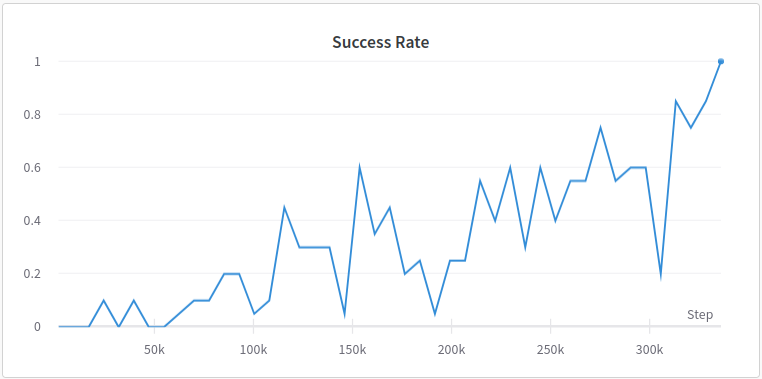
\includegraphics[width=\textwidth]{images/FPAPASR.png}
         \caption{Success Rate Plot for Current Implementation with Agent as Demonstrator.}
     \end{subfigure}
     \begin{subfigure}[b]{0.4\textwidth}
         \centering
         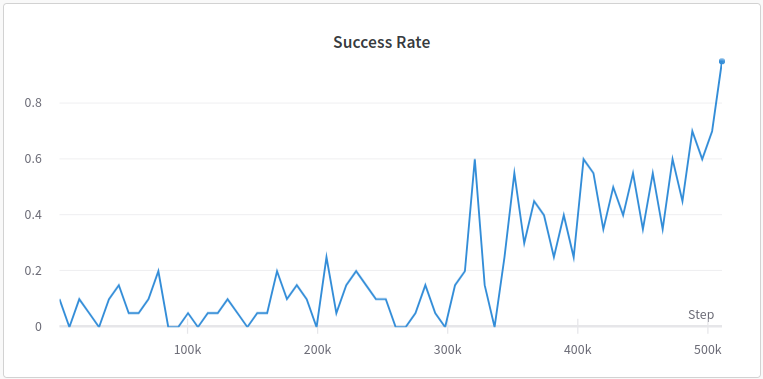
\includegraphics[width=\textwidth]{images/FPAPSSR.png}
         \caption{Success Rate Plot for Current Implementation with Script as Demonstrator.}
     \end{subfigure}
        \caption{Comparison Between Two Different Sources of Demonstrations.}
        \label{fig:CD}
\end{figure}

\begin{figure}[h!]
     \centering
     \begin{subfigure}[b]{0.4\textwidth}
         \centering
         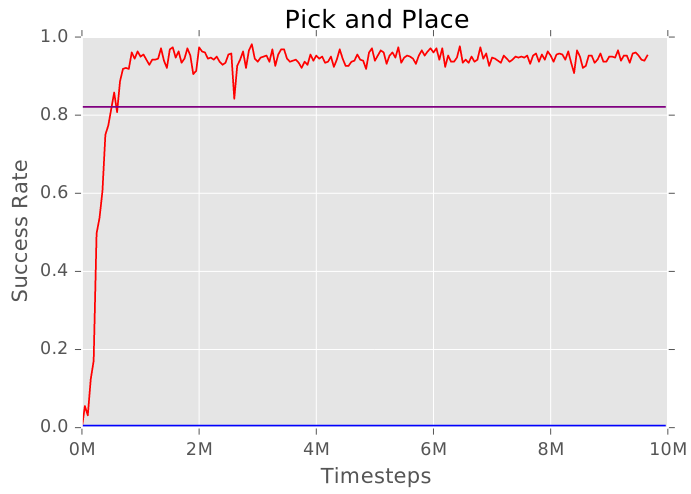
\includegraphics[width=\textwidth]{images/FPAPB.png}
         \caption{Success Rate Plot for \textcolor{blue}{Baseline 1}, \textcolor{red}{Baseline 2}, \textcolor{violet}{Baseline 3} \cite{nair2018overcoming}.}
     \end{subfigure}
     \begin{subfigure}[b]{0.4\textwidth}
         \centering
         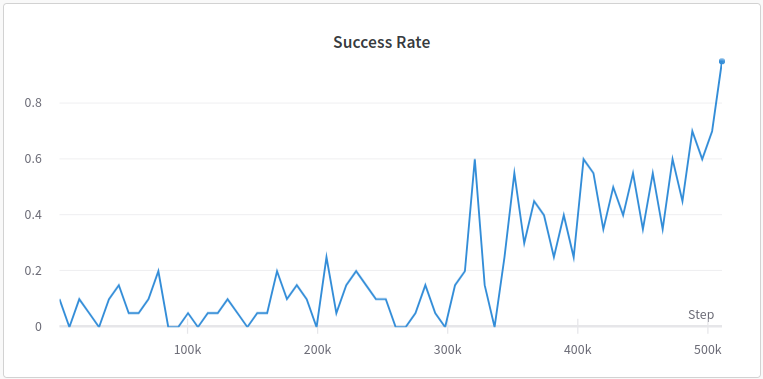
\includegraphics[width=\textwidth]{images/FPAPSSR.png}
         \caption{Success Rate Plot for Current Implementation with Script as Demonstrator.}
     \end{subfigure}
        \caption{Comparison Between Current Implementation with Different Demonstrations Source and Baselines 1, 2 and 3 for Fetch Pick and Place Task.}
        \label{fig:CDB}
\end{figure}

\begin{figure}[h!]
     \centering
     \begin{subfigure}[b]{0.4\textwidth}
         \centering
         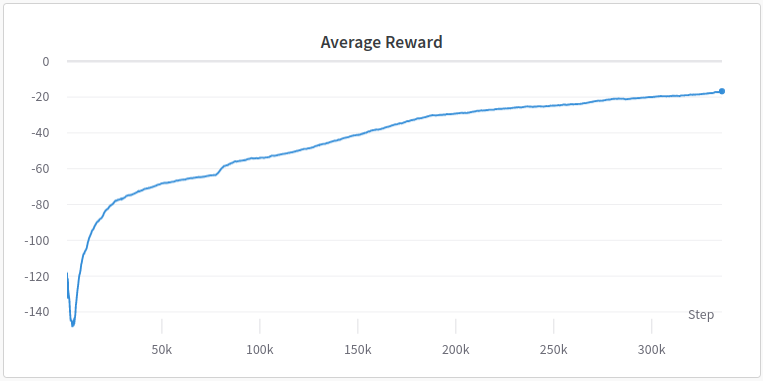
\includegraphics[width=\textwidth]{images/FPAPAAR.png}
         \caption{Average Reward Plot for Current Implementation with Agent as Demonstrator.}
     \end{subfigure}
     \begin{subfigure}[b]{0.4\textwidth}
         \centering
         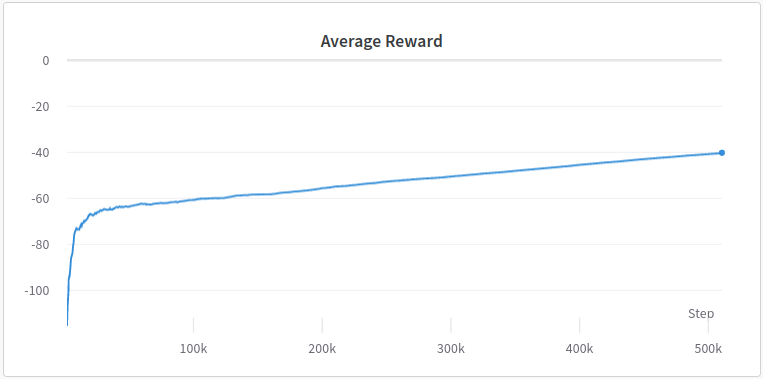
\includegraphics[width=\textwidth]{images/FPAPSAR.png}
         \caption{Average Reward Plot for Current Implementation with Script as Demonstrator.}
     \end{subfigure}
        \caption{Comparison Between Average Rewards for Different Demonstrations Sources.}
        \label{fig:CDAR}
\end{figure}

Figure \ref{fig:CD} shows the comparison between two different sources of demonstrations for the fetch pick and place environment. It is evident that even after varying the source of demonstrations the current implementation can successfully solve the environment. However, there are some interesting observations. The method using an agent as the demonstrator performs slightly better than the method that uses the handcrafted script as the demonstrator. The difference in convergence rate is not huge as a cause for concern but the noticeable difference has to be mentioned. The reason for this could be the ability of the demonstrator to complete the task and present rewards faster. On testing, it can be seen that even with external noise added the agent demonstrator can complete the task within 30 time steps out of the total 50 time steps limit per episode whereas the script takes around 40 time steps to complete the task. This delayed completion of the task could have influenced the learning agent to mimic similar behaviors as this method is behavior cloning after all. Figure \ref{fig:CDAR} shows the average reward for both the agents after a successful training session. From the figure, it can be seen that the agent which learned from the agent demonstrator has a higher average reward per episode compared to the agent which had the handcrafted script as the demonstrator. This observation further confirms the fact the slight delay in convergence time might be due to the agent mimicking the behavior of finishing the task later thus slowing down the training slightly. Even though there is a slight delay in training time between the two sources of demonstrations, both the sources can complete the task and provide accelerated learning compared to the previous baseline. \\

\subsection{Generalization Capability}

\begin{table}[h!]
\begin{tabular}{|c|c|c|}
\hline
Fetch Environment & Baseline 1 Test Success Rate & Current Implementation Test Success Rate \\ \hline
Reach          & 1.0 & 1.0 \\ \hline
Pick And Place & 0.8 & 0.9 \\ \hline
Push           & 0.8 & 0.9 \\ \hline
Slide          & 0.4 & 0.4 \\ \hline
\end{tabular}
\caption{Test Success Rate Comparison Between Current Implementation and Baseline 1.}
\label{tab:GC}
\end{table}

Table \ref{tab:GC} shows the test results of the trained agents for baseline 1 and the current implementation in all the environments. The success rates are calculated by averaging the success rate of a test set across 5 different random seeds. The current implementation can match the performance of baseline 1 in the reach and slide tasks and can outperform the baseline in the push and pick and place tasks. It can be observed that even though the current implementation can deliver good performance in the other environments it falls short in the slide task. It performs better than the baselines in training and equals the performance of the baseline in testing given the complexity of the environment this is not a bad result but definitely can be improved upon. As an extension of this research, it would be interesting to see if the transition from behavior cloning to complete reinforcement learning of the learned agent can deliver better performance. Using an agent trained using the current implementation and then using pure reinforcement learning to fine-tune the agent to try and see if it is possible to achieve better performance while still maintaining the accelerated learning. \\

\subsection{Number of Demonstrations Used}

\begin{table}[h!]
\begin{tabular}{|c|c|c|}
\hline
Fetch Environments & Demonstrations Baseline 2 & Demonstrations Current Implementation \\ \hline
Reach              & 100                     & 20                                    \\ \hline
Pick And Place     & 100                     & 40                                    \\ \hline
Push               & 100                     & 40                                    \\ \hline
Slide              & 100                     & 60                                    \\ \hline
\end{tabular}
\caption{Number of Demonstrations Used Compared to Baseline 2}
\label{tab:ND}
\end{table}

Table \ref{tab:ND} shows the number of demonstrations used for the current implementation compared to baseline 2 which uses a constant number of demonstrations for all the tasks. The current implementation can give better performance by using a lesser number of demonstrations. The number of demonstrations depends on the complexity of the task, which is the simple reach task needing only 20 demos, the average complexity environments of push and pick and place needing 40 demos, and the highly complex task of sliding needing 60 demos. The current implementation maintains the same number of demonstrations for the respective environments for both the sources of demonstrations used. If more demonstrations are available then well and good, but the current implementation can make do with lesser demons. Apart from the lesser number of demonstrations, as mentioned in the methodologies, adding external noise to the demons to replicate a more realistic approach in the collection of the demonstrations does not affect the performance of the agent, and the agent can do well with noisy demonstrations. As an extension to this research, it would be interesting to test this method with different combinations of demonstrations for example using a lesser number of high-quality demonstrations and a higher number of lower quality demonstrations. \\

\subsection{Model Complexity \textit{vs} Convergence Rate}

\begin{figure}[h!]
    \centering
    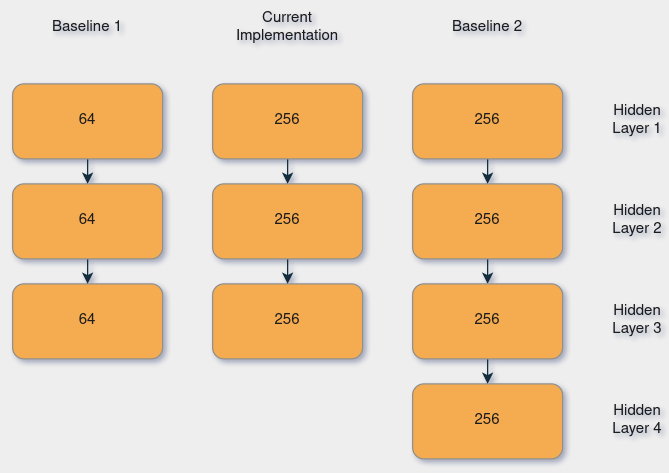
\includegraphics[width=\textwidth]{images/MAC.png}
    \caption{Model Architecture Comparison.}
    \label{fig:MAC}
\end{figure}

Figure \ref{fig:MAC} shows the comparison of the model complexity between the current implementations and the baselines. Baseline 1 was able to solve the tasks with relatively lesser model complexity of having 3 layers with 64 neurons in each layer. Both the current implementation and baseline 2 which use demos for learning have a higher model complexity, the baseline 2 having the highest of the lot with 4 layers and 256 neurons each while the current implementation has a slightly reduced version of the same with 3 layers and 256 neurons each. Baseline 1 has the highest convergence rate but the training time was reduced using powerful hardware resources, it uses no demonstrations and a random agent so it can get away with simple model complexity. Due to the use of demonstrations to prevent catastrophic forgetting of learned behaviors a higher complexity is required for baseline 2 and the current implementation, but the current implementation can perform better than the baseline 2 using a relatively lesser complex model, striking a good balance between the convergence rate and model complexity. \\

\subsection{Hardware Complexity \textit{vs} Training Time}

\begin{table}[h!]
\resizebox{\textwidth}{!}{%
\begin{tabular}{|c|ccc|ccc|ccc|}
\hline
Fetch Environment &
  Current Implementation &
   &
   &
  Baseline 1 &
   &
   &
  Baseline 4 &
   &
   \\ \hline
 &
  \multicolumn{1}{c|}{Hardware} &
  \multicolumn{1}{c|}{Training Time} &
  Success Rate &
  \multicolumn{1}{c|}{Hardware} &
  \multicolumn{1}{c|}{Training Time} &
  Success Rate &
  \multicolumn{1}{c|}{Hardware} &
  \multicolumn{1}{c|}{Training Time} &
  Success Rate \\ \cline{1-1} \cline{3-4} \cline{6-7} \cline{9-10} 
Reach &
  \multicolumn{1}{c|}{\begin{tabular}[c]{@{}c@{}}Intel i7-7th gen\\ 32Gb Ram\\ Gtx 1060 6Gb\end{tabular}} &
  \multicolumn{1}{c|}{0.1h} &
  1.0 &
  \multicolumn{1}{c|}{\begin{tabular}[c]{@{}c@{}}Distributed System\\ with 8 Parallel Workers\end{tabular}} &
  \multicolumn{1}{c|}{2.5h} &
  1.0 &
  \multicolumn{1}{c|}{-} &
  \multicolumn{1}{c|}{-} &
  - \\ \cline{1-1} \cline{3-4} \cline{6-7} \cline{9-10} 
Pick And Place &
  \multicolumn{1}{c|}{"} &
  \multicolumn{1}{c|}{3.0h} &
  1.0 &
  \multicolumn{1}{c|}{"} &
  \multicolumn{1}{c|}{2.5h} &
  0.0 &
  \multicolumn{1}{c|}{\begin{tabular}[c]{@{}c@{}}Intel i7-8th gen\\ 16Gb Ram\\ Gtx 1060 6Gb\end{tabular}} &
  \multicolumn{1}{c|}{3.0h} &
  0.6 \\ \cline{1-1} \cline{3-4} \cline{6-7} \cline{9-10} 
Push &
  \multicolumn{1}{c|}{"} &
  \multicolumn{1}{c|}{10.0h} &
  0.95 &
  \multicolumn{1}{c|}{"} &
  \multicolumn{1}{c|}{2.5h} &
  0.8 &
  \multicolumn{1}{c|}{-} &
  \multicolumn{1}{c|}{-} &
  - \\ \cline{1-1} \cline{3-4} \cline{6-7} \cline{9-10} 
Slide &
  \multicolumn{1}{c|}{"} &
  \multicolumn{1}{c|}{20.0h} &
  0.6 &
  \multicolumn{1}{c|}{"} &
  \multicolumn{1}{c|}{8h} &
  0.4 &
  \multicolumn{1}{c|}{-} &
  \multicolumn{1}{c|}{-} &
  - \\ \hline
\end{tabular}%
}
\caption{Comparison between the hardware's used between the current implementation and baselines.}
\label{tab:HC}
\end{table}

Table \ref{tab:HC} shows the hardware used by the current implementation and baseline 1 to solve the same set of tasks. Baseline 1 uses high-end hardware with a distributed system across 8 parallel workers running the environments and training the agent simultaneously. Even though the convergence rate for this baseline is higher, that is compensated by the use of powerful hardware showing more number time steps faster to the agent and solving the task with a much lesser training time. The current implementation and baseline 4 both use very modest hardware in the form of a laptop computer. The problem with baseline 4 is just a reward function is not enough for this complex environment, even though it can solve the task, the performance is just average. The current implementation using similar hardware can perform much better beating both baselines in all the tasks using modest hardware resources. It may not be the fastest in terms of training time but can deliver a low convergence rate. The agent can converge quickly with lesser interactions in the environment and seeing lesser states, striking a good balance in terms of hardware resources used and training time. \\

\section{Conclusion}

\subsection{Summary of Contributions}

The main focus of this research is investigating the different strategies to accelerate Reinforcement Learning. The exploration phase of Reinforcement Learning takes a big chunk of the overall training time and becomes increasingly difficult with more complex environments. Two strategies are explored to overcome this exploration. First is the use of demonstrations and training using a supervised approach. In this method, Behaviour Cloning which is a simple form of imitation learning is combined with a Reinforcement Learning agent, incorporating demonstrations into the training to overcome this exploration phase and accelerate the learning. A new loss function (a combination of losses from previous research)
\cite{nair2018overcoming} \cite{goecks2020integrating} is introduced along with a new training strategy which includes a pre-training phase and a different way of presenting the data to the agent. The loss function is designed in such a way that the agent is not limited or constrained by the demo behaviours and is free to develop new behaviours and grow beyond the demo actions. The noise was added to the demonstrations and different sources of the demonstrations were tested to show that this method can cope with change and also with suboptimal demos and still perform well. The second strategy is the use of a simple and informative reward function to further support accelerated learning. The research was careful not to implement an over-engineered and complex reward function which might lead to suboptimal behaviour and has stuck to simplicity. The only drawback is the availability of demonstrations as this method relies on demos to work, but other than that if demos are available this research offers a simple and straightforward implementation compared to other researches in the same domain. The proposed method can perform much better than previous related baselines while striking a good balance between model complexity and convergence rate, also hardware complexity and training time, providing a middle ground in this complex domain. \\

\subsection{Summary of Results}
\begin{table}[h!]
\centering
\begin{tabular}{|c|cc|cc|c|}
\hline
Fetch Environment & Baseline I               &      & Current Implementation    &      & Speedup   \\ \hline
 & \multicolumn{1}{c|}{Timesteps} & Success Rate & \multicolumn{1}{c|}{Timesteps} & Success Rate &  \\ \hline
Reach             & \multicolumn{1}{c|}{150K} & 1.0  & \multicolumn{1}{c|}{16K}  & 1.0  & $\sim$9x  \\ \hline
Pick and Place    & \multicolumn{1}{c|}{10M} & 0.0  & \multicolumn{1}{c|}{310K} & 1.0  & -         \\ \hline
Push              & \multicolumn{1}{c|}{10M} & 0.85 & \multicolumn{1}{c|}{1.1M} & 0.95 & $\sim$10x \\ \hline
Slide             & \multicolumn{1}{c|}{10M} & 0.4  & \multicolumn{1}{c|}{2M}   & 0.6  & $\sim$5x  \\ \hline
\end{tabular}
\caption{Comparison of Current Implementation with Baseline 1}
\label{tab:my-table1}
\end{table}

\begin{table}[h!]
\centering
\begin{tabular}{|c|cc|cc|c|}
\hline
Fetch Environment & Baseline II             &     & Current Implementation    &      & Speedup  \\ \hline
               & \multicolumn{1}{c|}{Timesteps} & Success Rate & \multicolumn{1}{c|}{Timesteps} & Success Rate &          \\ \hline
Reach             & \multicolumn{1}{c|}{-}  & -   & \multicolumn{1}{c|}{16K}  & 1.0  & -        \\ \hline
Pick and Place & \multicolumn{1}{c|}{1M}        & 0.9          & \multicolumn{1}{c|}{310K}      & 1.0          & $\sim$3x \\ \hline
Push              & \multicolumn{1}{c|}{3M} & 0.9 & \multicolumn{1}{c|}{1.1M} & 0.95 & $\sim$3x \\ \hline
Slide             & \multicolumn{1}{c|}{8M} & 0.6 & \multicolumn{1}{c|}{2M}   & 0.6  & $\sim$4x \\ \hline
\end{tabular}
\caption{Comparison of Current Implementation with Baseline 2}
\label{tab:my-table2}
\end{table}

\begin{table}[h!]
\centering
\begin{tabular}{|l|l|l|}
\hline
Fetch Environment & Baseline III   & Current Implementation \\ \hline
                  & Success Rate & Success Rate           \\ \hline
Reach             & -            & 1.0                    \\ \hline
Pick and Place    & 0.8          & 1.0                    \\ \hline
Push              & 0.2          & 0.95                   \\ \hline
Slide             & 0.2          & 0.6                    \\ \hline
\end{tabular}
\caption{Comparison of Current Implementation with Baseline 3}
\label{tab:my-table}
\end{table}

The highlights of the results for the current implementation are, for the same environment suite when compared to previous related results this implementation can provide a much better convergence rate showing accelerated learning. Baseline 1 was the first to solve these complex environments but with a high convergence rate. This was compensated by using high-end hardware resources in the form of distributed computing and also in the form of some environment-related tricks to solve the more complex tasks. Baseline 2 performs much better showcasing the advantages of the current implementation. Baseline 3 is more of a hit or miss, this is one of the main problems of pure Behaviour Cloning methods, either they can solve the task very well or struggle badly. This entirely depends upon the source, quality and quantity of the demonstrations. Also using only pure dense reward functions can solve the task but not provide a good accuracy. This is where the current implementation can outperform the baselines by combining Behaviour Cloning with Reinforcement Learning and dense reward functions. Also, the fetch push task was able to develop new behaviours which have both positive and negative outcomes. The negative is that even though the task is solved successfully this behaviour might be okay within a simulation but may not be a desired behaviour for the real world. The positive is that apart from solving the tasks successfully and providing accelerated learning, the current implementation can outperform the demos and also develop new behaviours. Apart from the straightforward implementation, the training was performed in using modest hardware resources on a laptop computer providing a middle ground in the form of a framework to solve complex tasks. \\

\subsection{Answering Research Questions}

\begin{itemize}[leftmargin=0.7in]
    \item[Q1.  ] \textbf{Can the proposed method successfully solve complex robotics tasks?} \\

    \item[A1.  ] The current implementation can successfully solve all the tasks in the complex multi-goal tasks in the fetch robotics environment suite with a success rate and faster convergence rate across all the tasks. \\

    \item[Q2.  ] \textbf{Does the proposed method achieve accelerated learning without a compromise to generalization or resulting in any undesirable outcomes?} \\
    
    \item[A2.  ] The current implementation can provide accelerated learning across all the environments without any loss in generalization. After training the current implementation was tested across 5 different random seed test environments and has good performance very close to that of the training results, except for the fetch slide environment which has the highest complexity of the lot, but these results were within margin when compared to the baselines. For three environments the resultant behaviour was as expected, but for the fetch push task even though the task was solved successfully, the resultant behaviour might be suitable for a simulation but not desirable for the real world. This is not a major cause for concern, the reason is explained in the results section and this problem can be solved as an extension to this research. \\
    
    \item[Q3.  ] \textbf{Does the source, quality and quantity of the demonstrations used matter for performance?} \\
    
    \item Two different sources of demonstrations were tested with the current implementation and the observation is that the sources of demonstrations do impact performance, but not in a way that the algorithm is unusable. The observations have been presented in the results section and the summary is that both the sources of demonstrations were able to outperform the baselines. The noise was added to the demonstrations and both success and failure cases were shown to the agent and the agent was able to learn and perform well from these suboptimal demonstrations. Finally compared to the baselines the current implementation uses a fewer number of demonstrations but this number depends on the complexity of the environment but is overall lesser than the baselines. \\

    \item[Q4.  ] \textbf{How does the proposed method compare to previous related baselines?} \\
    
    \item In terms of convergence rate the current implementation performs much better than the related baselines. Some of the methods compensate for this by either using complex implementations or high-end hardware resources reducing the training time. The current implementation can provide a balance between implementation simplicity and modest hardware resources used. The only drawback is there has to be some form of demonstrations available as this method is heavily reliant on the demos and will not work without them. \\
\end{itemize}

\subsection{Future Work}

As an extension to this research, it would be interesting to explore a few other aspects to either solve some existing condition or observe something new. The first and most important area is to address the different emergent behaviour for the fetch push environment. As mentioned earlier the task is solved successfully and it might be an okay result for the simulation but not a desirable action for the real world. This can be solved by either changing the soft-constrains dynamics of the environment or adding a term in the reward function to change the desired behaviour, these related areas can be explored. The second would be to improve performance in complex tasks like the fetch slide environment. This can be done by transitioning from Behaviour Cloning to Reinforcement Learning completely. The current method uses a fixed ratio of Behaviour Cloning and Reinforcement Learning losses, but it would be interesting to see this approach of first learning using Behaviour Cloning and then slowly transitioning to Reinforcement Learning and then using pure Reinforcement Learning to further continue the training to fine-tune the performance and learning. It would be interesting to see if there is any improvement in the performance and if any new behaviours are observed and in the slide environment if the max success rate threshold can be beaten. The third would be playing with the demonstrations, trying out different sources, also changing the quality and the number of demonstrations. A higher number of lower quality demonstrations or a lower number of higher quality demonstrations can be tried out and the performance can be studied. Finally, it would be interesting to extend this current implementation to other multi-goal environments, related to robotics like hand-manipulation, or sequential-goals related to robotics like stacking blocks, or non-robotics related tasks like walking, running, balancing, etc \cite{brockman2016openai}. \\

\pagestyle{contents}

\bibliographystyle{ieeetr}
\bibliography{biblio}

\pagestyle{appendix}
\appendix
\section*{Appendices}
\addcontentsline{toc}{section}{Appendices}
\renewcommand{\thesubsection}{\Alph{subsection}}

\subsection{Additional Graphs}

\begin{figure*}[h!]
    \centering
    \begin{subfigure}[b]{0.4\textwidth}
        \centering
        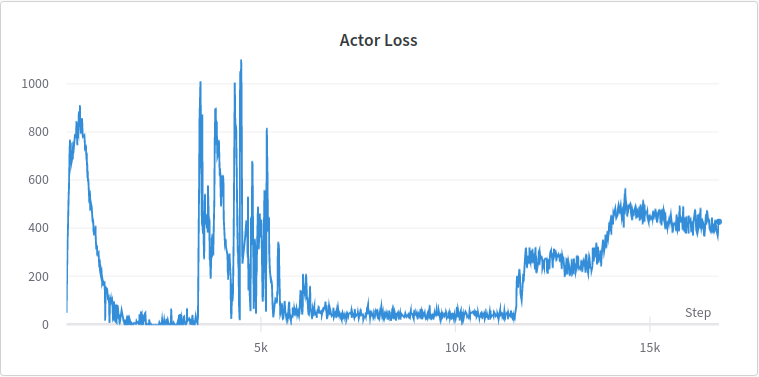
\includegraphics[width=\textwidth]{images/FRAL}
        \caption[Network2]%
        {{\small Actor Loss}}    
        \label{fig:mean and std of net14}
    \end{subfigure}
    \hfill
    \begin{subfigure}[b]{0.4\textwidth}  
        \centering 
        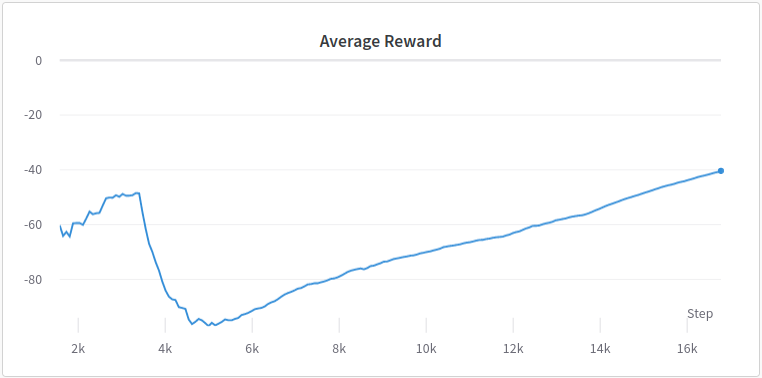
\includegraphics[width=\textwidth]{images/FRAR}
        \caption[]%
        {{\small Average Reward}}    
        \label{fig:mean and std of net24}
    \end{subfigure}
    \vskip\baselineskip
    \begin{subfigure}[b]{0.4\textwidth}   
        \centering 
        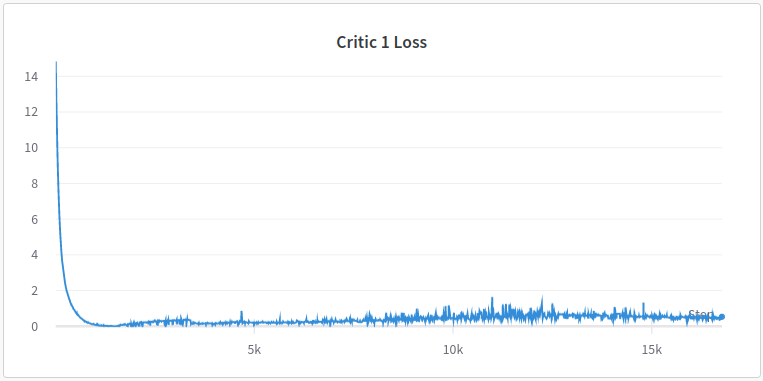
\includegraphics[width=\textwidth]{images/FRC1L.png}
        \caption[]%
        {{\small Critic 1 Loss}}    
        \label{fig:mean and std of net34}
    \end{subfigure}
    \hfill
    \begin{subfigure}[b]{0.4\textwidth}   
        \centering 
        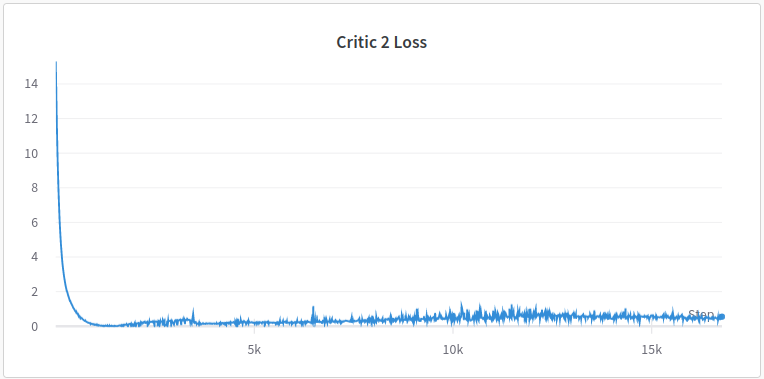
\includegraphics[width=\textwidth]{images/FRC2L.png}
        \caption[]%
        {{\small Critic 2 Loss}}    
        \label{fig:mean and std of net44}
    \end{subfigure}
    \caption[ Rewards and Loss Plots for the Fetch Reach Environment. ]
    {\small Rewards and Loss Plots for the Fetch Reach Environment.} 
    \label{fig:mean and std of nets}
\end{figure*}

\begin{figure*}[h!]
    \centering
    \begin{subfigure}[b]{0.4\textwidth}
        \centering
        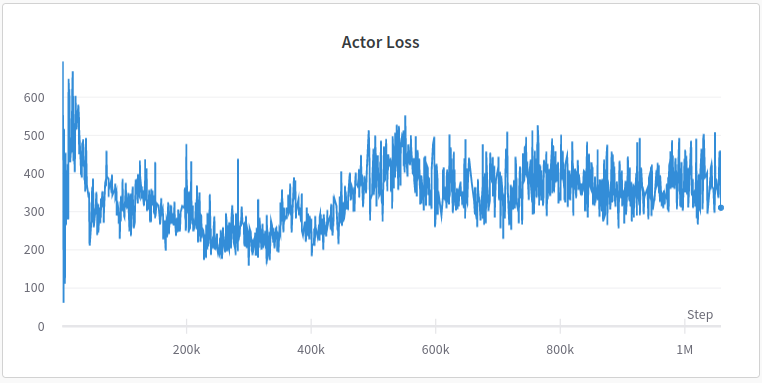
\includegraphics[width=\textwidth]{images/FPAL}
        \caption[Network2]%
        {{\small Actor Loss}}    
        \label{fig:mean and std of net14}
    \end{subfigure}
    \hfill
    \begin{subfigure}[b]{0.4\textwidth}  
        \centering 
        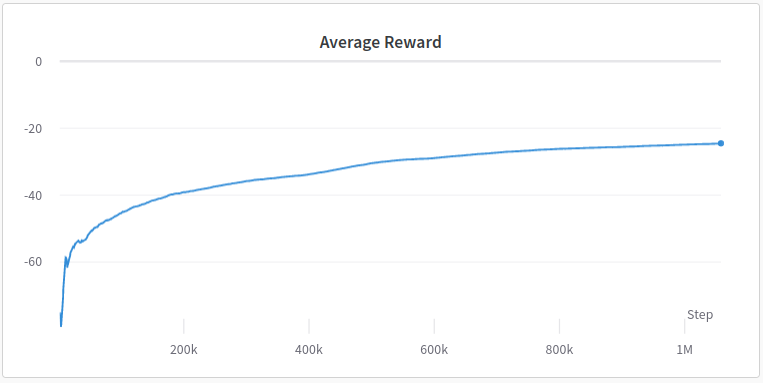
\includegraphics[width=\textwidth]{images/FPAR}
        \caption[]%
        {{\small Average Reward}}    
        \label{fig:mean and std of net24}
    \end{subfigure}
    \vskip\baselineskip
    \begin{subfigure}[b]{0.4\textwidth}   
        \centering 
        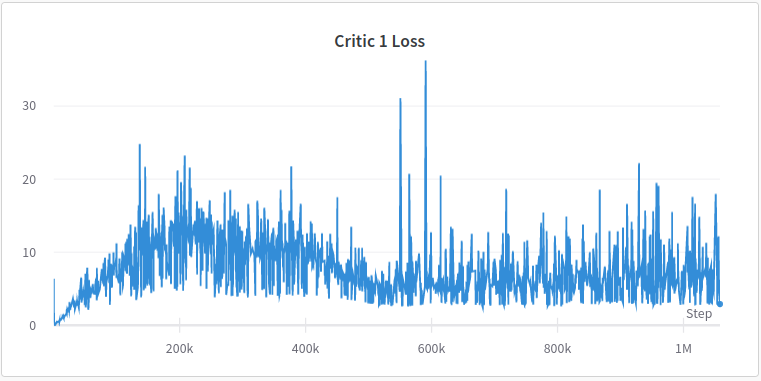
\includegraphics[width=\textwidth]{images/FPC1L.png}
        \caption[]%
        {{\small Critic 1 Loss}}    
        \label{fig:mean and std of net34}
    \end{subfigure}
    \hfill
    \begin{subfigure}[b]{0.4\textwidth}   
        \centering 
        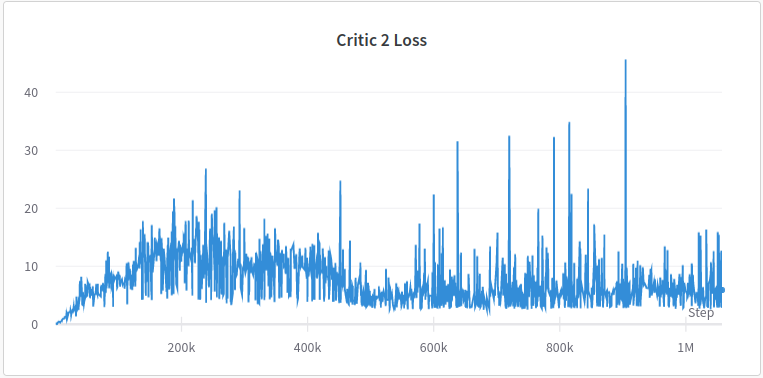
\includegraphics[width=\textwidth]{images/FPC2L.png}
        \caption[]%
        {{\small Critic 2 Loss}}    
        \label{fig:mean and std of net44}
    \end{subfigure}
    \caption[ Rewards and Loss Plots for the Fetch Push Environment. ]
    {\small Rewards and Loss Plots for the Fetch Push Environment.} 
    \label{fig:mean and std of nets}
\end{figure*}

\begin{figure*}[h!]
    \centering
    \begin{subfigure}[b]{0.475\textwidth}
        \centering
        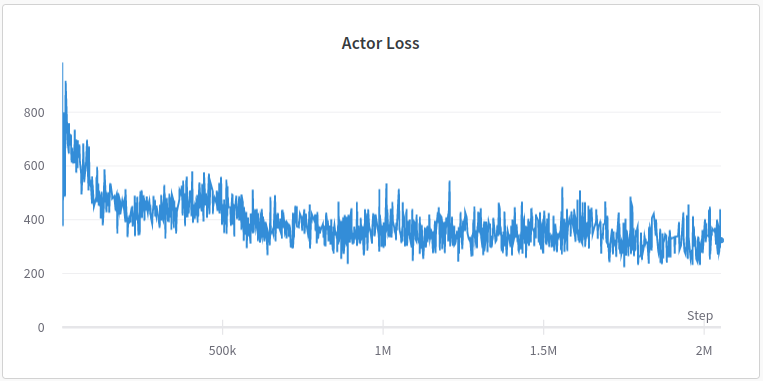
\includegraphics[width=\textwidth]{images/FSAL}
        \caption[Network2]%
        {{\small Actor Loss}}    
        \label{fig:mean and std of net14}
    \end{subfigure}
    \hfill
    \begin{subfigure}[b]{0.475\textwidth}  
        \centering 
        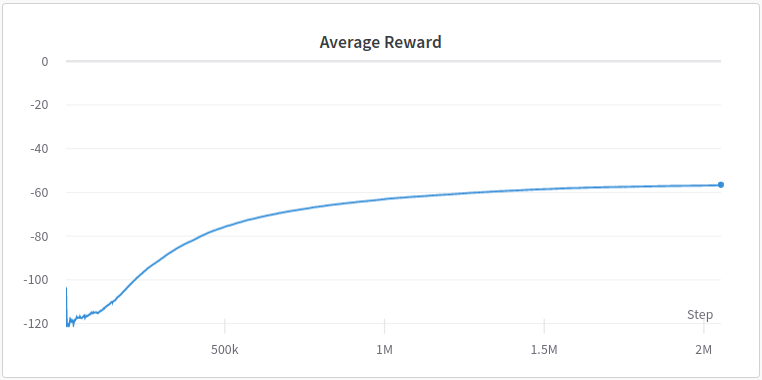
\includegraphics[width=\textwidth]{images/FSAR}
        \caption[]%
        {{\small Average Reward}}    
        \label{fig:mean and std of net24}
    \end{subfigure}
    \vskip\baselineskip
    \begin{subfigure}[b]{0.475\textwidth}   
        \centering 
        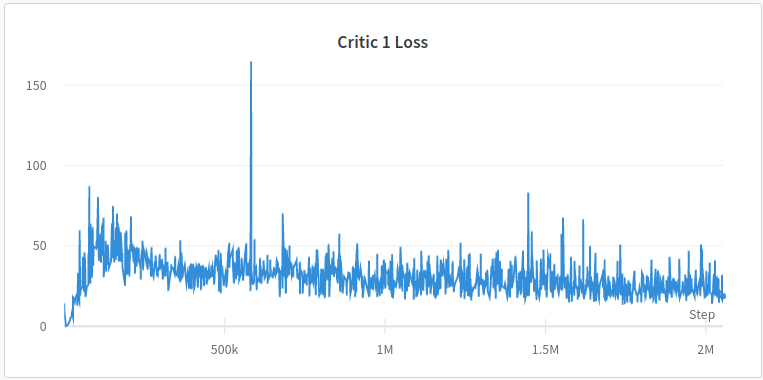
\includegraphics[width=\textwidth]{images/FSC1L.png}
        \caption[]%
        {{\small Critic 1 Loss}}    
        \label{fig:mean and std of net34}
    \end{subfigure}
    \hfill
    \begin{subfigure}[b]{0.475\textwidth}   
        \centering 
        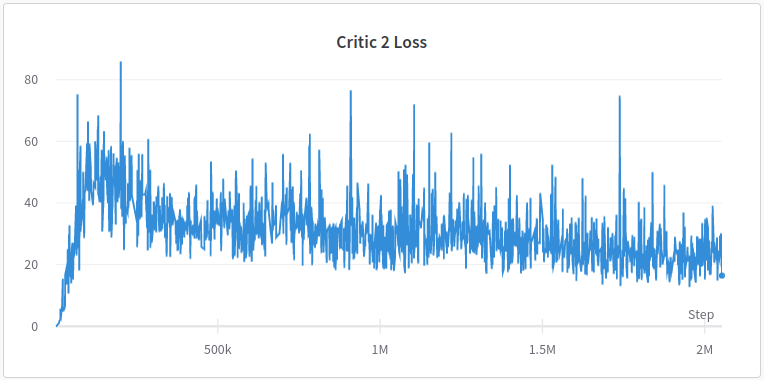
\includegraphics[width=\textwidth]{images/FSC2L.png}
        \caption[]%
        {{\small Critic 2 Loss}}    
        \label{fig:mean and std of net44}
    \end{subfigure}
    \caption[ Rewards and Loss Plots for the Fetch Slide Environment. ]
    {\small Rewards and Loss Plots for the Fetch Slide Environment.} 
    \label{fig:mean and std of nets}
\end{figure*}

\begin{figure*}[h!]
    \centering
    \begin{subfigure}[b]{0.475\textwidth}
        \centering
        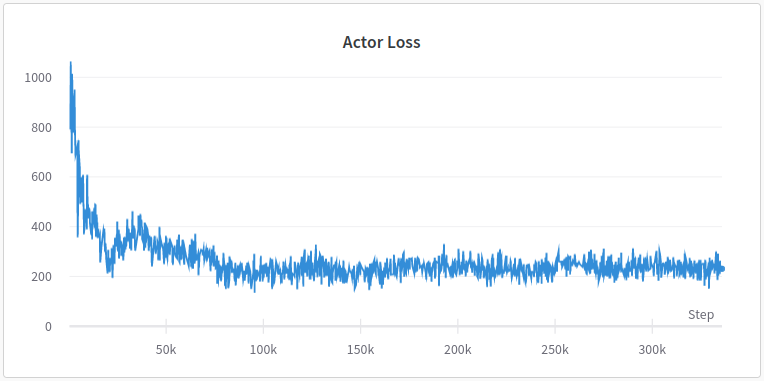
\includegraphics[width=\textwidth]{images/FPAPAAL.png}
        \caption[Network2]%
        {{\small Actor Loss}}    
        \label{fig:mean and std of net14}
    \end{subfigure}
    \vskip\baselineskip
    \begin{subfigure}[b]{0.475\textwidth}   
        \centering 
        \includegraphics[width=\textwidth]{images/FPAPAC1L.png}
        \caption[]%
        {{\small Critic 1 Loss}}    
        \label{fig:mean and std of net34}
    \end{subfigure}
    \hfill
    \begin{subfigure}[b]{0.475\textwidth}   
        \centering 
        \includegraphics[width=\textwidth]{images/FPAPAC2L.png}
        \caption[]%
        {{\small Critic 2 Loss}}    
        \label{fig:mean and std of net44}
    \end{subfigure}
    \caption[ Rewards and Loss Plots for the Fetch Pick and Place Environment with Agent Demonstrator. ]
    {\small Rewards and Loss Plots for the Fetch Pick and Place Environment with Agent Demonstrator.} 
    \label{fig:mean and std of nets}
\end{figure*}

\begin{figure*}[h!]
    \centering
    \begin{subfigure}[b]{0.475\textwidth}
        \centering
        \includegraphics[width=\textwidth]{images/FPAPSAL.png}
        \caption[Network2]%
        {{\small Actor Loss}}    
        \label{fig:mean and std of net14}
    \end{subfigure}
    \vskip\baselineskip
    \begin{subfigure}[b]{0.475\textwidth}   
        \centering 
        \includegraphics[width=\textwidth]{images/FPAPSC1L.png}
        \caption[]%
        {{\small Critic 1 Loss}}    
        \label{fig:mean and std of net34}
    \end{subfigure}
    \hfill
    \begin{subfigure}[b]{0.475\textwidth}   
        \centering 
        \includegraphics[width=\textwidth]{images/FPAPSC2L.png}
        \caption[]%
        {{\small Critic 2 Loss}}    
        \label{fig:mean and std of net44}
    \end{subfigure}
    \caption[ Rewards and Loss Plots for the Fetch Pick and Place Environment with Script Demonstrator. ]
    {\small Rewards and Loss Plots for the Fetch Pick and Place Environment with Script Demonstrator.} 
    \label{fig:mean and std of nets}
\end{figure*}


\end{document}